% Author: Sandy Burden, Version 1
% ----------------------------------------------------------------
% NIASRA Beamer template for Slides *******************************
% ----------------------------------------------------------------
\documentclass{beamer}
%\documentclass[handout]{beamer}
%\pgfpagesuselayout{4 on 1}[a4paper, border shrink=5mm, landscape]

\usepackage{color}
\usepackage{pgfpages}
\usepackage{graphicx}
\usepackage[utf8]{inputenc}
\usepackage[T1]{fontenc}
\usepackage{amsmath,amsthm, amssymb}
\usepackage{amsfonts}
\usepackage{natbib}
\usepackage{bm}
\usepackage{hyperref}
\usepackage{hyphenat}
\pdfmapfile{+sansmathaccent.map}

\hfuzz5pt % Don't bother to report over-full boxes < 5pt
\vfuzz5pt % Don't bother to report over-full boxes < 5pt
\setlength{\parskip}{3mm}
\usetheme{NIASRA}

% Include secheader option if you want section headers at top of slide.  Can get wide...
%\usetheme[secheader]{NIASRA}

\newcommand{\Yt}{\widetilde{Y}}
\newcommand{\Deltab} {\boldsymbol{\Delta}}
\newcommand{\intd} {\mathrm{d}}
\newcommand{\Bmat} {\textbf{B}}
\newcommand{\Dmat} {\textbf{D}}
\newcommand{\Qmat} {\textbf{Q}}
\newcommand{\Cmat} {\textbf{C}}
\newcommand{\cmat} {\textbf{c}}
\newcommand{\Imat} {\textbf{I}}
\newcommand{\bvec} {\textbf{b}}
\newcommand{\svec} {\textbf{s}}
\newcommand{\uvec} {\textbf{u}}
\newcommand{\omegab} {\boldsymbol {\omega}}
\newcommand{\s}{\mathbf{s}}
\newcommand{\h}{\mathbf{h}}
\renewcommand{\b}{\mathbf{b}}
\newcommand{\z}{\mathbf{z}}
\renewcommand{\v}{\mathbf{v}}
\renewcommand{\u}{\mathbf{u}}
\newcommand{\w}{\mathbf{w}}
\renewcommand{\d}{\mathrm{d}}
\newcommand{\Z}{\mathbf{Z}}
\newcommand{\x}{\mathbf{x}}
\newcommand{\Y}{\mathbf{Y}}
\newcommand{\Yvec}{\mathbf{Y}}
\newcommand{\Zvec}{\mathbf{Z}}
\newcommand{\epsilonb}{\boldsymbol{\varepsilon}}
\newcommand{\bI}{\mathbf{I}}
\newcommand{\bB}{\mathbf{B}}
\newcommand{\bbeta}{\boldsymbol{\beta}}
\newcommand{\thetab}{\boldsymbol{\theta}}
\newcommand{\bzero}{\boldsymbol{0}}
\newcommand{\bSigma}{\bm{\Sigma}}
\newcommand{\E}{E}
\newcommand{\cov}{\mathrm{cov}}
\newcommand{\var}{\mathrm{var}}
\newcommand{\tr}{\mathrm{tr}}
\newcommand{\diag}{\mathrm{diag}}
\newcommand{\vect}{\mathrm{vec}}
\newcommand{\Gau}{\mathrm{Gau}}
\newcommand{\RR}{\mathbb{R}}
\newcommand{\varthetab} {{\boldsymbol{\vartheta}}}
\newcommand{\Dist}{\mathrm{Dist}}

\newcommand{\red}{\textcolor{red}}%
\newcommand{\blue}{\textcolor{blue}}

 \title[Multivariate Spatial Modelling]{A Conditional Approach to Multivariate Spatial Modelling}
% \subtitle{``An application to flux estimation"} %Not required if you don't want it
 \author[N. Cressie \& A. Zammit-Mangion]{Noel Cressie \\ and \\ Andrew Zammit-Mangion} %
  \institute[]{National Institute for Applied Statistics Research Australia \\  University of Wollongong \\ \vspace{0.4in} 
\includegraphics[height=1cm]{NiasraUowLonghand}} % Substitute date of presentation or include todays date instead.
\date{}
\begin{document}

\begin{frame}
\titlepage
\end{frame}

% The following slide provides a table of contents for the presentation.  Include or leave out as required.  Additional contents for individual sections can be included throughout the presentation using \tableofcontents[currentsection] or currentsubsection or hideallsubsections, subsubsectionstyle=hide etc.


\begin{frame}
\frametitle{Introduction}

\begin{itemize}
\item \textcolor{red}{Univariate} spatial model \vfill
\begin{itemize}
	\item ``Marginal'' behaviour of a single spatial variable\vfill
	\item Optimally predict at all spatial locations: \textcolor{red}{Kriging} \vfill
\end{itemize}
\item \textcolor{red}{Multivariate} spatial model \vfill
\begin{itemize}
    \item Two or more interacting spatial variables \vfill
    \item Optimally predict one of the variables by using the observations on all variables: \textcolor{red}{Cokriging} \vfill
    \item Determine which variable caused the observed phenomenon: \textcolor{red}{Source separation}\vfill 
\end{itemize}\vfill
\end{itemize}

\end{frame}

% ###################

\begin{frame}
\frametitle{Example: Ozone and Max Temperature}

\cite{RoyleBerliner1999}, Midwestern USA, centred on Illinois, Lake Michigan, and Chicago (Left panel: Tropospheric ozone concentrations in ppb. Right panel: Maximum temperature in degC)

\begin{center}
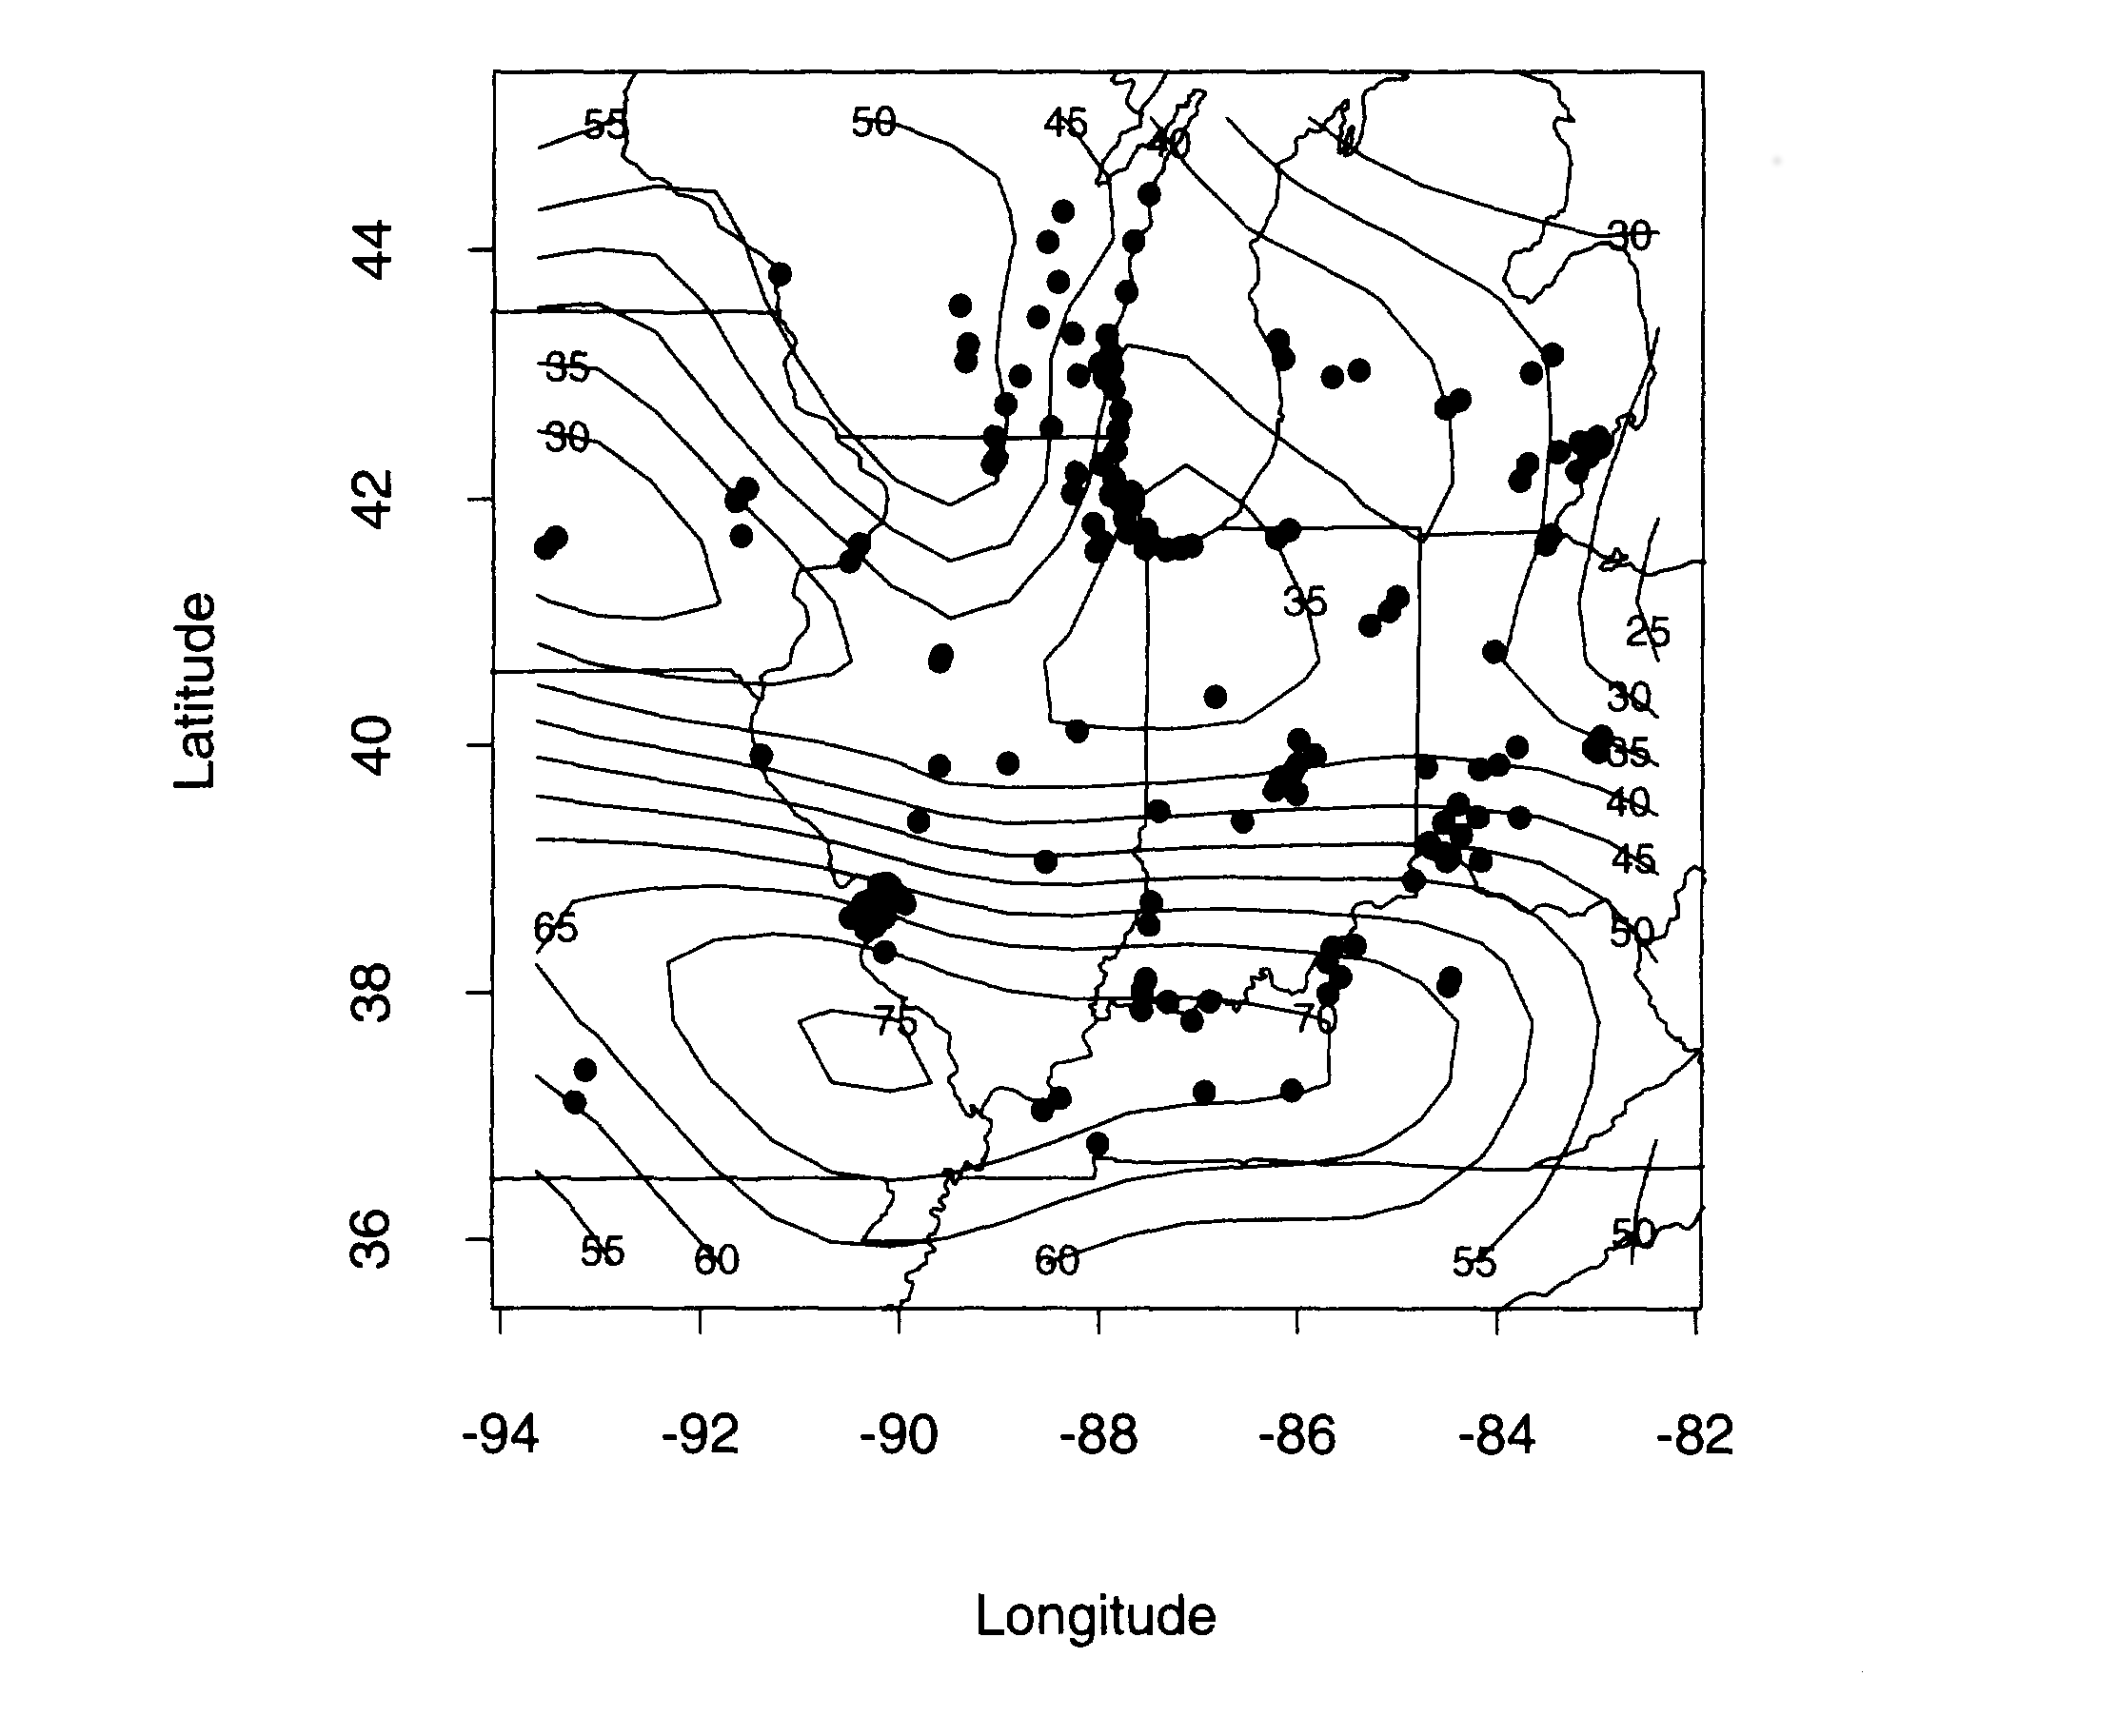
\includegraphics[width=2.5in]{./ozone.png}
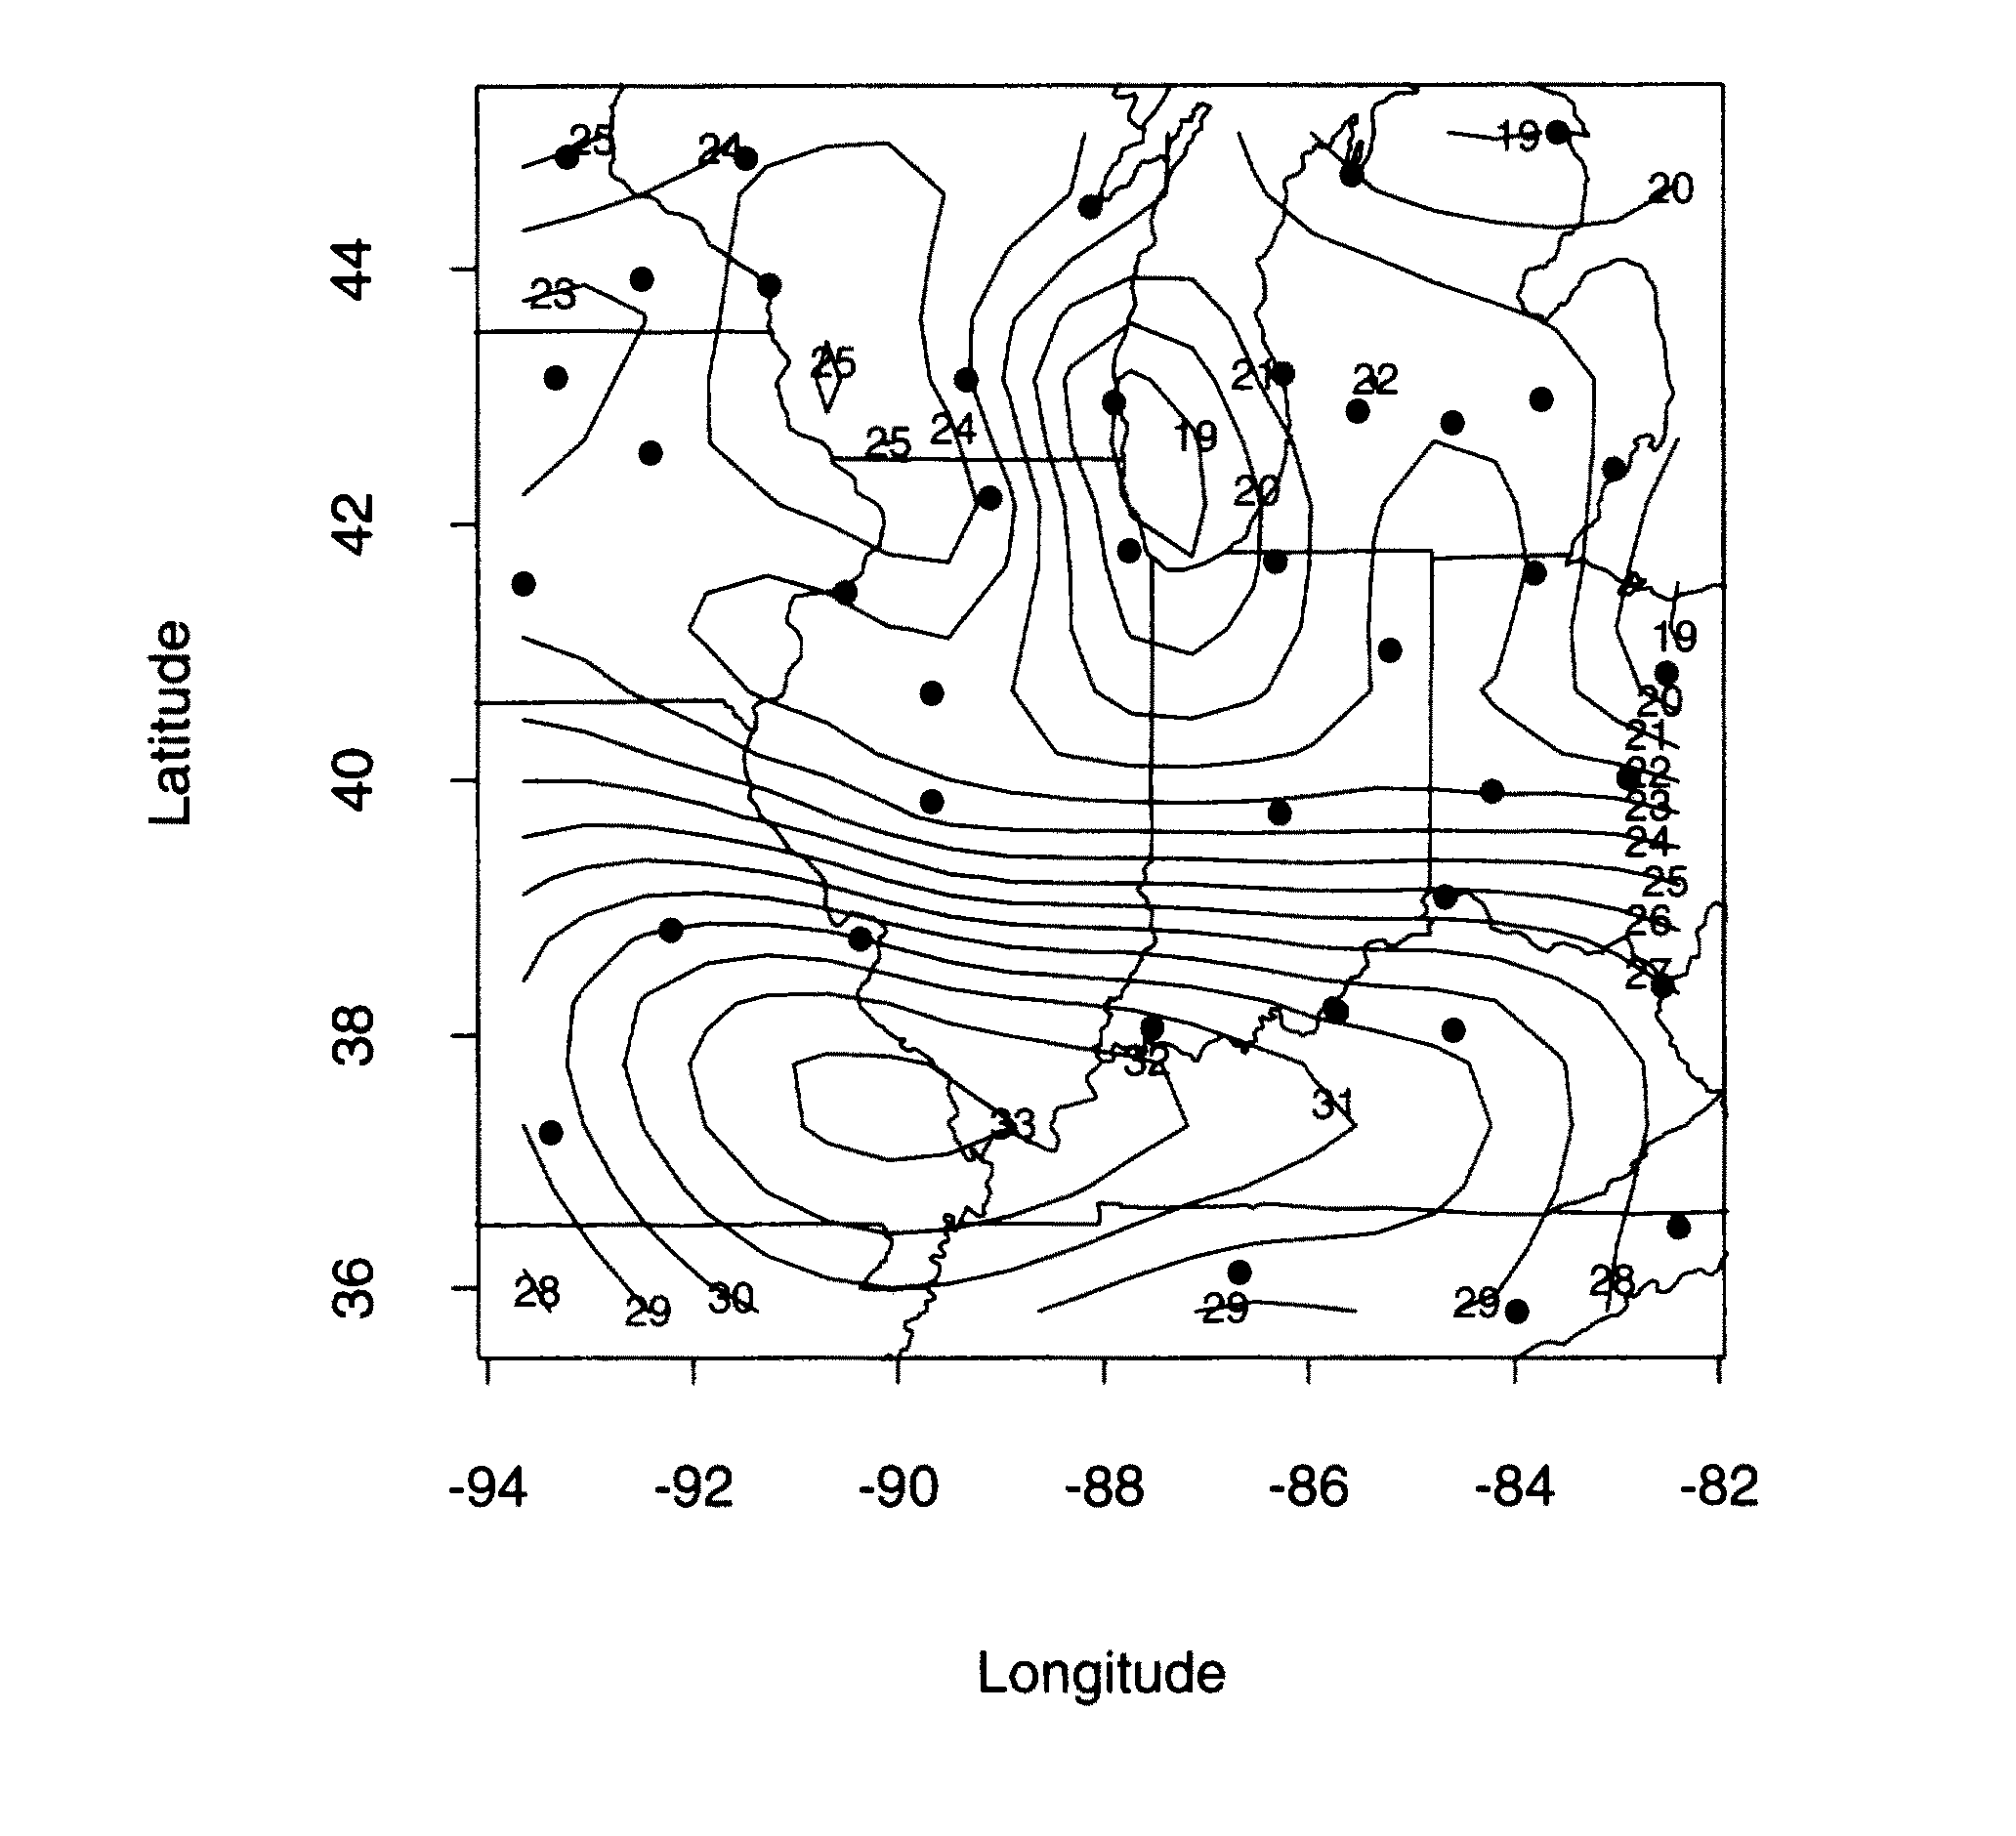
\includegraphics[width=2.3in]{./maxt.png}
\end{center}
\end{frame}

\begin{frame}
\frametitle{Example: Temperature and Pressure}
\cite{Gneitingetal2010}, North American Pacific Northwest (Left panel: Forecast temperature errors. Right panel: Forecast pressure errors)

\begin{center}
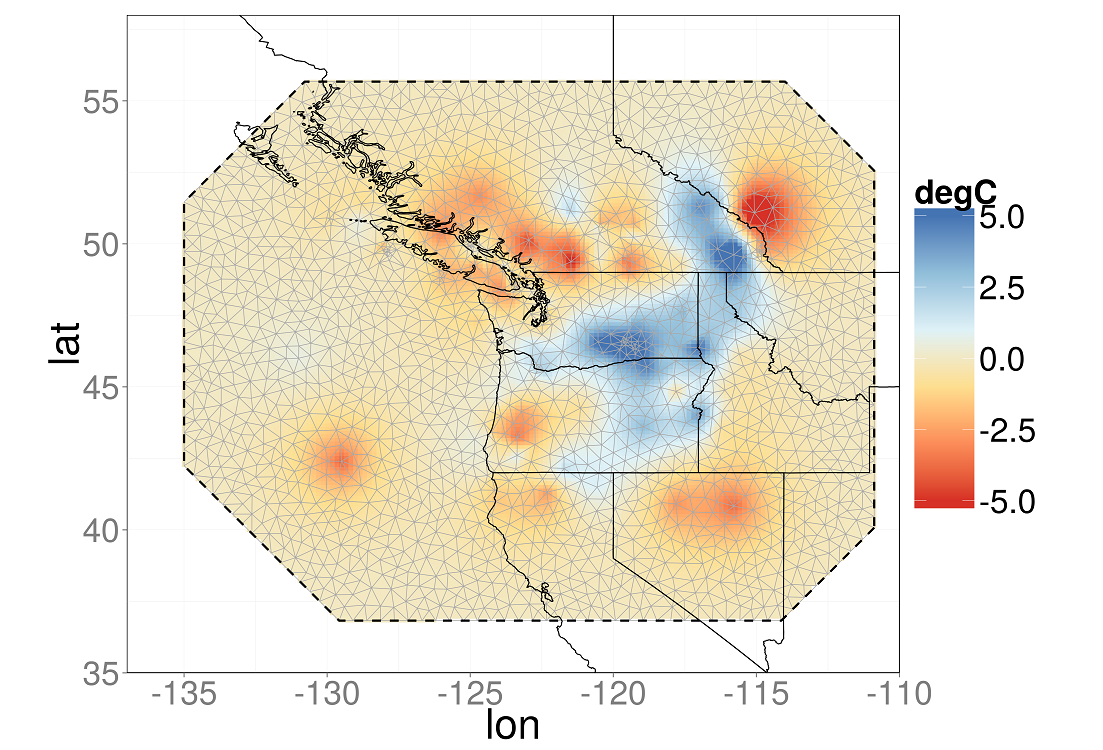
\includegraphics[width=2.5in]{./Temp.png}
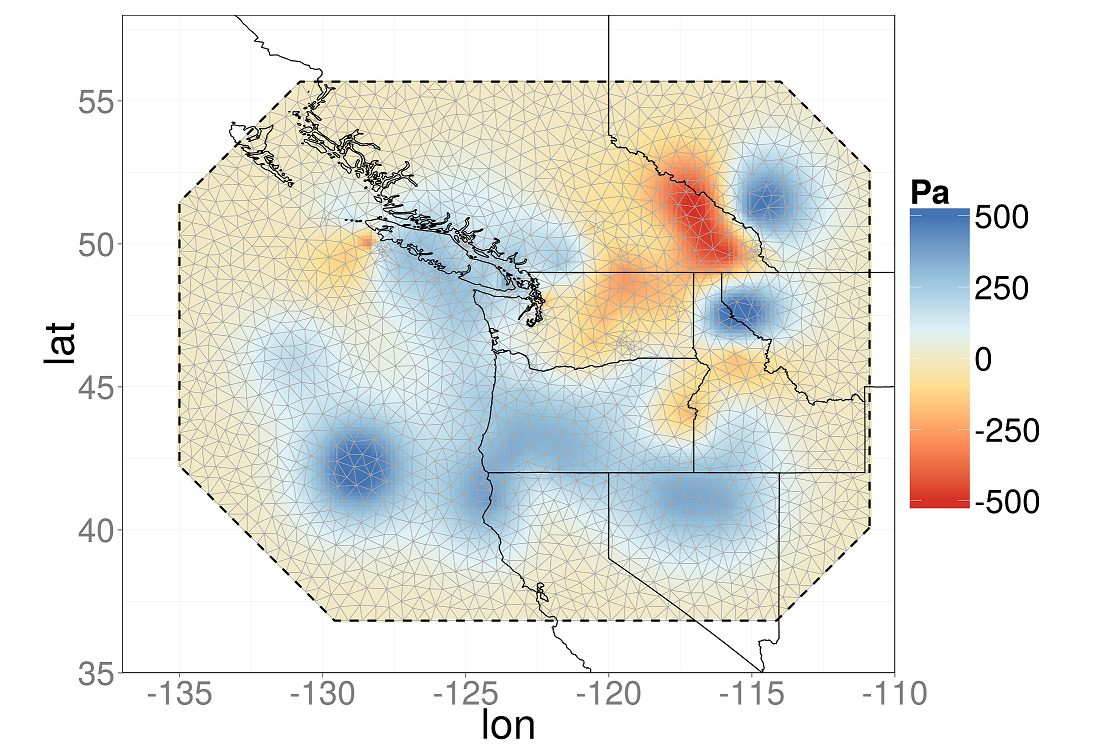
\includegraphics[width=2.3in]{./Pressure.png}
\end{center}
\end{frame}

% ###################

\begin{frame}
\frametitle{The challenge}

\begin{itemize}
\item \textcolor{red}{Statistical Modelling}: Given a bivariate process $(Y_1(\cdot), Y_2(\cdot))$, we say that the \emph{cross-covariance function matrix} (\textcolor{red}{CCFM}),
\begin{equation*}
\label{eq1}
\left(\begin{array}{cc} C_{11}(\cdot,\cdot) & C_{12}(\cdot,\cdot) \\ C_{21}(\cdot,\cdot) & C_{22}(\cdot,\cdot)\end{array} \right),
\end{equation*}
is \textcolor{red}{nonnegative-definite (nnd)} if \textcolor{red}{any} covariance matrix derived from it is nnd. In the CCFM,
$$
C_{ij}(\s,\u)\equiv\cov(Y_i(\s),Y_j(\u));\,\s,\u\in\mathbb{R}^d.
$$
\item \textcolor{red}{Computational}: Sometimes we have computational difficulty with kriging (univariate models) -- how do such algorithms scale to multivariate modelling and \textcolor{red}{multivariate spatial prediction} (including cokriging)? %\vfill
\end{itemize}
\end{frame}

% ###################

%\subsection{Current approaches}

\begin{frame}
\frametitle{Current approaches}

\begin{itemize}
\item \textcolor{red}{Linear model of co-regionalisation}, or LMC \citep{JournelHuijbregts1978, Wackernagel1995}: Define
\begin{align*}
    Y_1(\cdot) &\equiv a_{11}\Yt_1(\cdot) + a_{12}\Yt_2(\cdot),\\
    Y_2(\cdot) &\equiv a_{21}\Yt_1(\cdot) + a_{22}\Yt_2(\cdot),
\end{align*}
where, independently,
\begin{align*}
    \Yt_1(\cdot) &\sim \mathcal{N}(\mu_1(\cdot), C_{1}(\cdot,\cdot)),\\
    \Yt_2(\cdot) &\sim \mathcal{N}(\mu_2(\cdot), C_{2}(\cdot,\cdot)).
\end{align*}
\end{itemize}
The CCFM is nnd for any $\{a_{ij}: i,j = 1,2\}$, and 
$$
C_{ij}(\cdot,\cdot) = a_{i1}a_{j1}C_{1}(\cdot,\cdot) + a_{i2}a_{j2}C_{2}(\cdot,\cdot).
$$ 
Hence, $C_{ij}(\s,\u)=C_{ji}(\s,\u)=C_{ij}(\u,\s)$. This \textcolor{red}{symmetry constraint} can be inappropriate.

\end{frame}

% ###################

\begin{frame}
\frametitle{Multivariate Mat\'{e}rn models}
Multivariate Mat\'{e}rn models can be built from the assumption that $\{C_{ij}(\mathbf{h}):\mathbf{h}\in\mathbb{R}^d\}$ are each proportional to a \textcolor{red}{univariate Mat\'{e}rn correlation function}; that is,
$$
C_{ij}(\mathbf{h})\propto 2^{1-\nu_{ij}}\Gamma(\nu_{ij})^{-1}(\kappa_{ij}\|\mathbf{h}\|)^{\nu_{ij}}K_{\nu_{ij}}(\kappa_{ij}\|\mathbf{h}\|),
$$
where $\{\nu_{ij}\}$ are smoothness parameters, and $\{\kappa_{ij}\}$ are spatial-scale parameters. The proportionality constants are given by a covariance matrix $\{\tau_{ij}\}$. Restrictions on parameters are needed to obtain a CCFM that is nnd. 

Consider now the \textcolor{red}{bivariate Mat\'{e}rn} models:
%Note that \textcolor{red}{asymmetry} (i.e., $C_{12}(\s,\u)\neq C_{21}(\s,\u)$) can occur.
\vfill
\end{frame}

\begin{frame}
\frametitle{Current approaches, ctd}
\cite{Gneitingetal2010} defined bivariate Mat\'{e}rn models, however they satisfy the symmetry constraint, $C_{ij}(\s,\u)=C_{ji}(\s,\u)$.
\begin{itemize}
\item \textcolor{red}{Bivariate parsimonious Matérn model}: Suppose that $\nu_{ij}\equiv(\nu_i+\nu_j)/2$ and $\kappa_{ij}\equiv\kappa;i,j=1,2$. In $\mathbb{R}^2$, the CCFM is nnd iff
$$
\frac{\tau_{12}^2}{\tau_{11}\tau_{22}}\leq\frac{\nu_1\nu_2}{((\nu_1+\nu_2)/2)^2}.
$$

  %Let $C^o(\cdot)$ be a generic stationary, isotropic covariance function. Define
%\begin{align}
   %C_{ij}^o(\cdot) & \equiv \beta_{ij}M(\cdot; \nu_{ij}, \kappa_{ij}),
%\end{align}
%where $M(\cdot)$ is a stationary, isotropic Matérn covariance function. 

%Let $\kappa_{ii} = \kappa_{ij} = \kappa$ and set $\nu_{ij} = (\nu_{ii} + \nu_{jj})/2$. Then if the matrix  $(\beta_{ij}:i,j = 1,2)$ is positive-definite, the CCFM is positive-definite.\vfill

\item \textcolor{red}{Bivariate full Matérn model}:  Here assumptions on smoothness and spatial-scale parameters are relaxed, but finding the parameters for which the CCFM is nnd is much more involved.\vfill
\end{itemize}
\vfill
\end{frame}

% ###################
%\begin{frame}
%\frametitle{Current approaches (limitations)}
%\begin{itemize}
%\item Stuck with homogeneous, often stationary and isotropic models\vfill
%\item Stuck with fixed scales (parsimonious Matérn) \vfill
%\item Stuck with Matérn models (e.g., full Matérn models) \vfill
%\item Stuck with symmetry (e.g., LMC). \vfill
%\end{itemize}
%\end{frame}
% ###################

\begin{frame}
\frametitle{Symmetry is usually inappropriate}
Often one process ($Y_{1}(\cdot)$) ``lags'' the other ($Y_2(\cdot)$). If this is the case, we should not use models that have the symmetry constraint.
\begin{itemize}
\item $Y_1(\cdot)$: precipitation at present.
\item $Y_2(\cdot)$: precipitation in 5-minutes time.
\end{itemize}
The \textcolor{red}{symmetry constraint}, $C_{12}(\s,\u)=C_{21}(\s,\u)$, is \textcolor{red}{inappropriate} here.
\vspace{-0.5cm}

\begin{center}
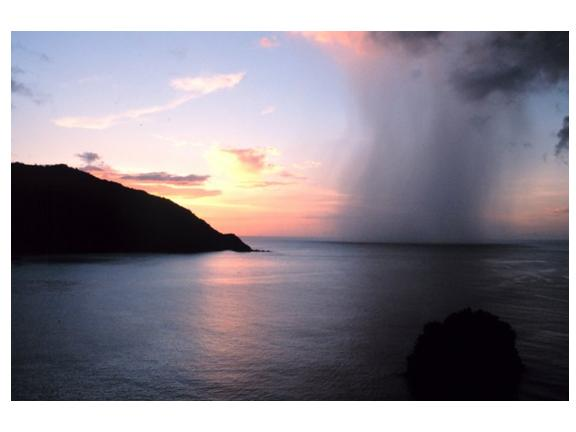
\includegraphics[width=2.5in]{rain.png}
\end{center}
\end{frame}

% ###################

\begin{frame}
\frametitle{Bivariate spatial models with asymmetry}

\begin{itemize}
\item An easy way to introduce asymmetry is to consider $Y_1(\cdot)$ and $Y_2(\cdot)$ modelled with the symmetry constraint, and then \textcolor{red}{shift} one of the processes by $\Deltab$ (e.g., fit the model $Y_1(\cdot)$ and $Y_2(\cdot-\Deltab)$. 
\newline References: \cite{VerHoefCressie1993,ChristensenAmemiya2001,ChristensenAmemiya2002,Li_2011}
\vfill
\item Another approach is to introduce latent dimensions. Then asymmetry in the full-dimensional space implies asymmetry in the original space. Reference:~\cite{Apanasovich_2010}
\end{itemize}
\vfill
\end{frame}

% ###################

%\subsection{Bivariate models}

\begin{frame}
\frametitle{A conditional approach}
This approach is valid regardless of whether $Y_1(\cdot)$ is the baseline process or whether $Y_2(\cdot)$ is. It is often obvious which one lags and which one leads. Here we choose $Y_1(\cdot)$ as the baseline (i.e., $Y_1(\cdot)$ lags) with covariance function $C_{11}(\cdot,\cdot)$. Write:
\begin{align*}
\E\left(Y_2(\s)\mid Y_1(\cdot)\right)&\,=\int_D{\textcolor{red}{b(\s,\v)}Y_1(\v)\,\d \v};\quad \s\in D,\\
\cov\left(Y_2(\s),Y_2(\u)\mid Y_1(\cdot)\right)&\,=\textcolor{red}{C_{2\mid 1}(\s,\u)};\quad \s,\u\in \mathbb{R}^d.
\end{align*}
Building blocks:
\begin{itemize}
\item $C_{11}(\cdot,\cdot)$ (\textcolor{red}{univariate} covariance); nnd function
\item $C_{2|1}(\cdot,\cdot)$ (\textcolor{red}{univariate} covariance); nnd function
\item $b(\cdot,\cdot)$ (\textcolor{red}{interaction} function); any integrable function
\end{itemize}
\end{frame}

% ###################

\begin{frame}
\frametitle{Properties}
\begin{itemize}
\item The CCFM is easy to find:
$$
\begin{bmatrix} C_{11}(\s,\u) & \int_DC_{11}(\s,\v)\textcolor{red}{b(\u,\v)}\d\v \\ \int_D\textcolor{red}{b(\s,\v)}C_{11}(\v,\u)\d\v & ~~~~~C_{22}(\s,\u)\end{bmatrix},
$$
where 
$$
C_{22}(\s,\u) = \textcolor{red}{C_{2\mid 1}(\s,\u)}+\int_D\int_D \red{b(\s,\v)}C_{11}(\v,\w) \red{b(\w,\u)}\d\v\d\w,
$$
and it is \textcolor{red}{always nnd} (the proof is given later). \vfill

\item \textcolor{red}{Asymmetry} (i.e., $C_{12}(\svec,\uvec) \ne C_{21}(\svec,\uvec)$) is guaranteed if $b(\cdot,\cdot)$ is not symmetric (i.e., $b(\s,\u)\neq b(\u,\s)$, for some $\s,\u$).\vfill
\end{itemize}
\end{frame}

% ###################

\begin{frame}
\frametitle{Properties, ctd}
\vspace{-.5cm}
A small example of asymmetry in $\mathbb{R}^1$:
\begin{itemize}
\item Define $b^o(s-u) \equiv b(s,u)$ that is off-centre (i.e., not symmetric about 0).
\item $s,u \in \{-1, -0.9 ,\dots,0.9, 1\}$.
\item From the figure, $C_{22}(\cdot,\cdot)$ has edge effects and $\textcolor{red}{C_{12}(s,u)\neq C_{21}(s,u)}$; see the figure below.
\end{itemize}
\vspace{-.9cm}
\begin{center}
\hfill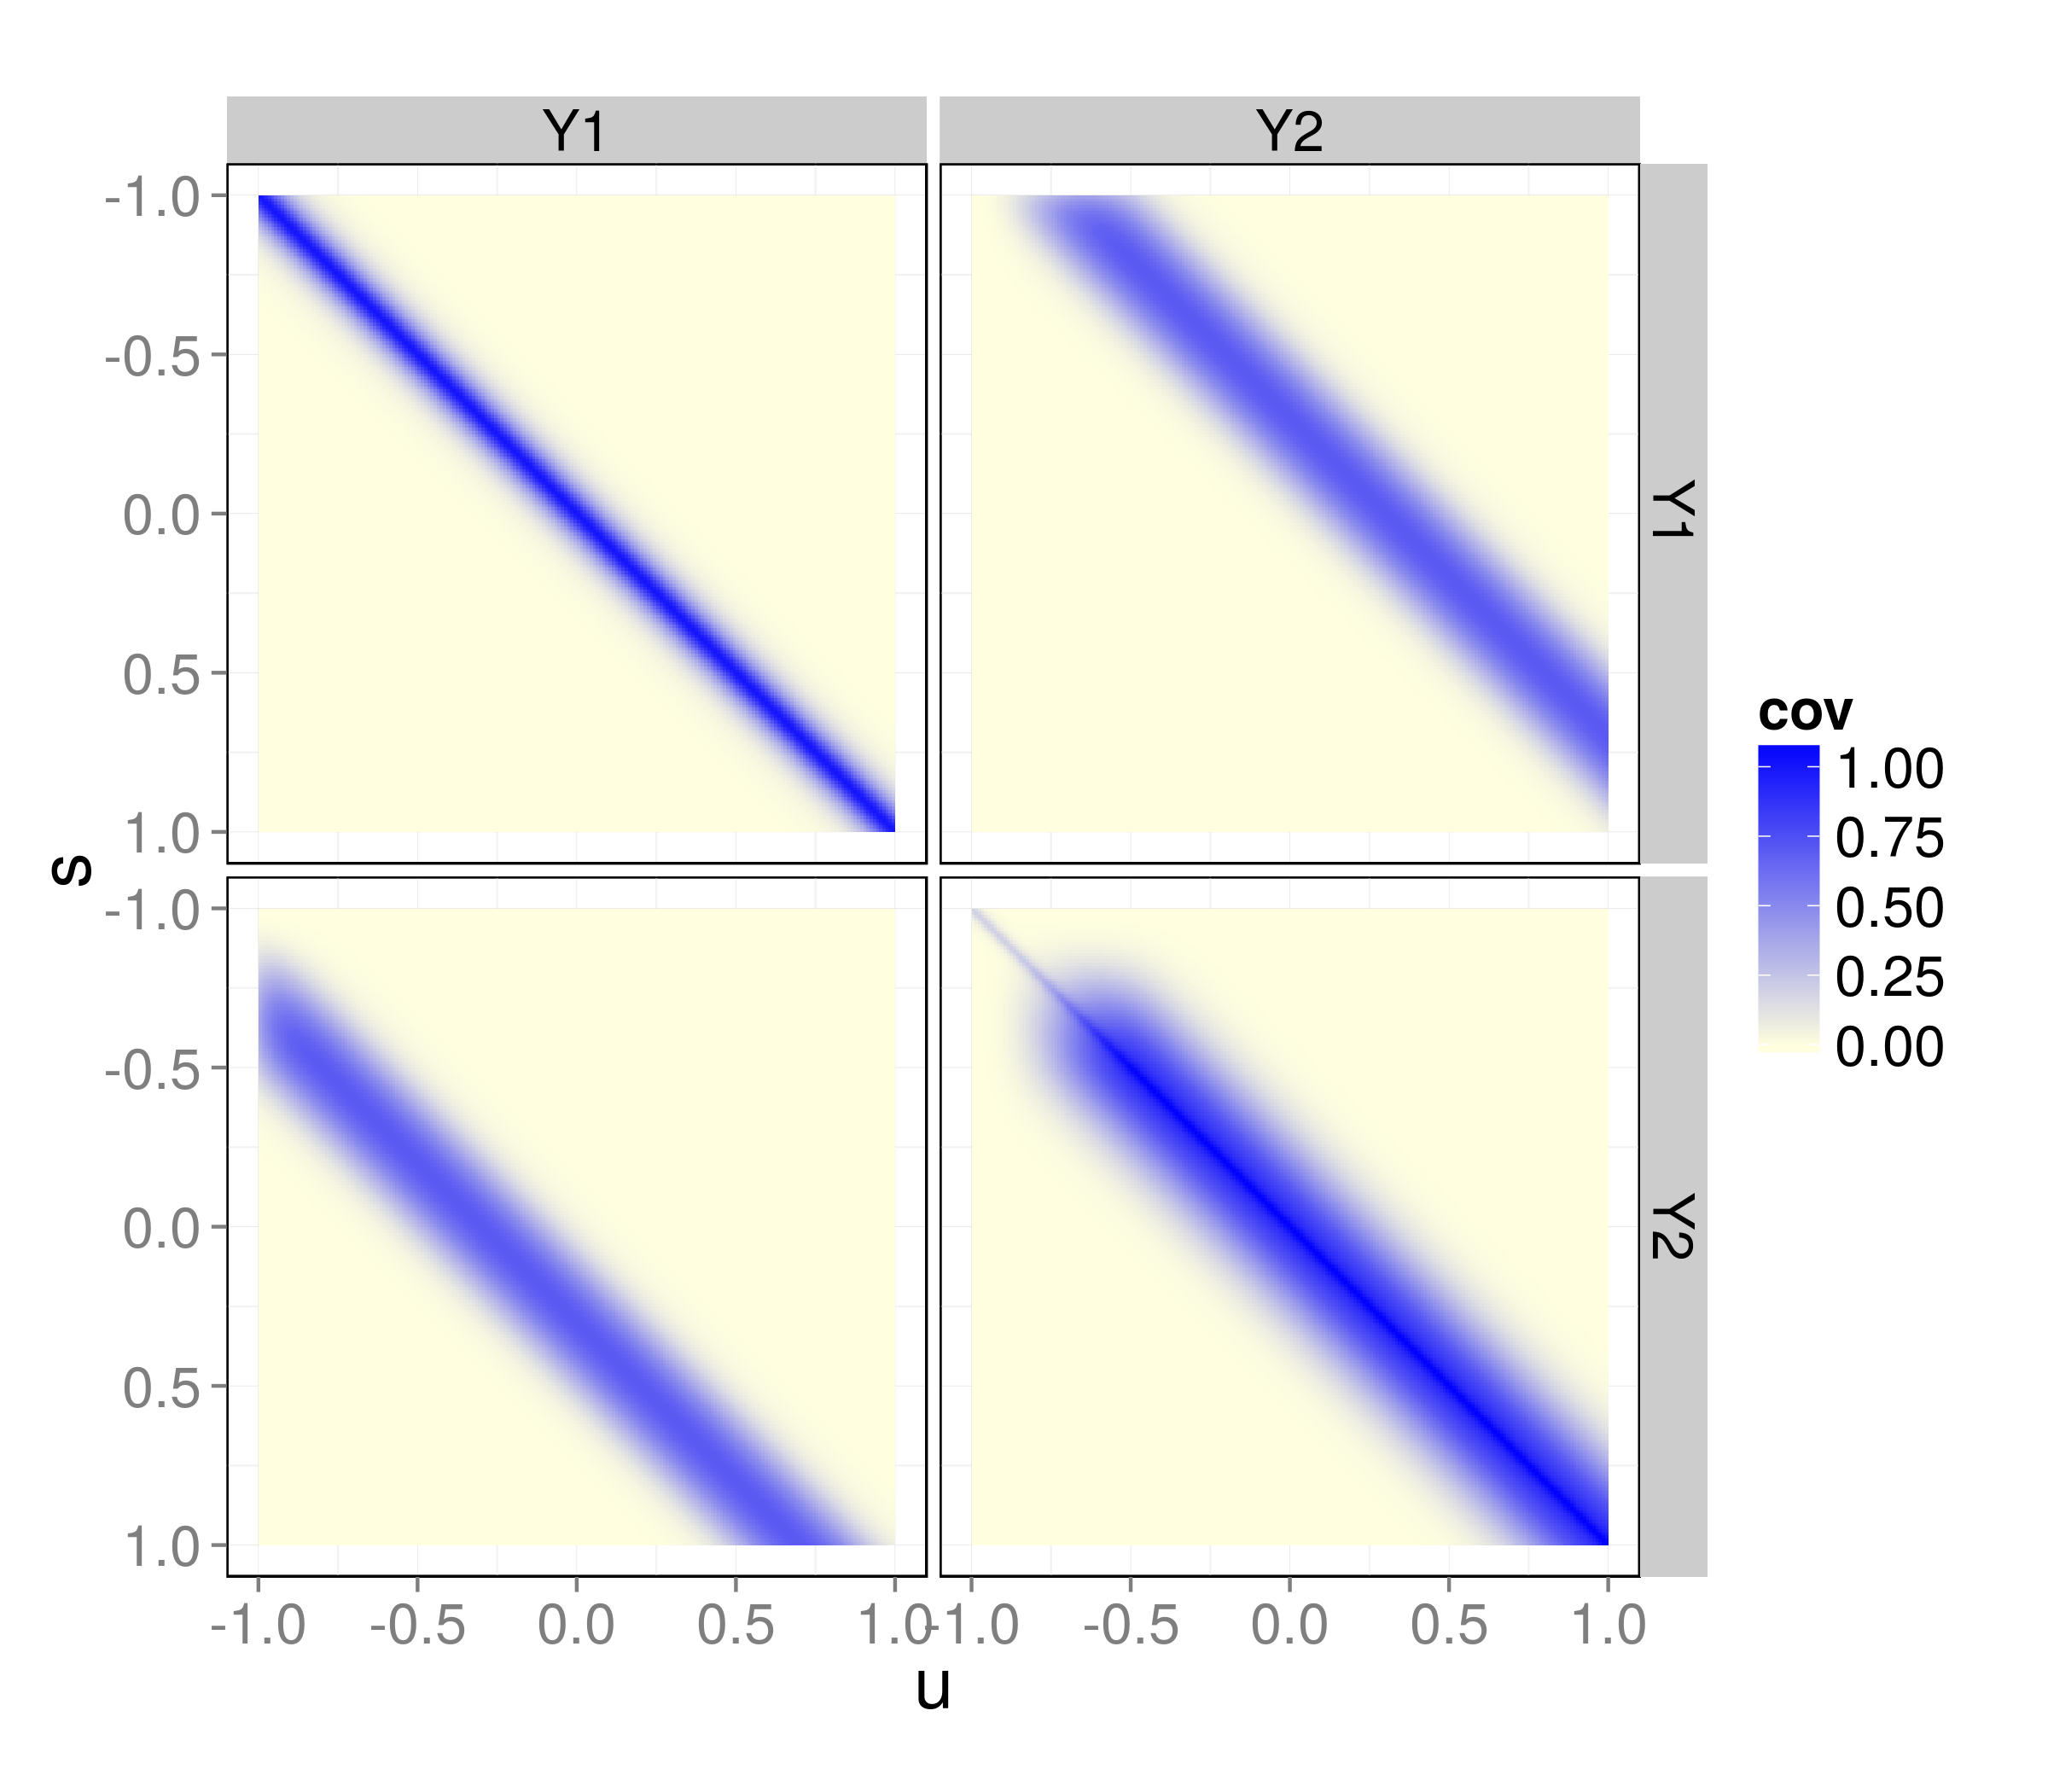
\includegraphics[width=2.5in]{Sigma.png}
\end{center}
\end{frame}

% ###################

\begin{frame}
\frametitle{Properties, ctd}
A conditional approach to multivariate spatial modelling:
\begin{itemize}
\item Generally, we can have \textcolor{red}{heterogeneity}, since $C_{11}(\cdot,\cdot)$, $C_{2|1}(\cdot,\cdot)$ need not be stationary, and $b(\svec,\uvec)$ need not be symmetric in $\svec$ and $\uvec$. \vfill

\item We are \textcolor{red}{not restricted to Matérn fields}. The bivariate parsimonious Matérn model is a \textcolor{red}{special case}.\vfill

\item $Y_2(\cdot)$ can be \textcolor{red}{arbitrarily smoother} than $Y_1(\cdot)$ and it can have a \textcolor{red}{different spatial scale}.\vfill

\end{itemize}
\end{frame}

% ###################

\begin{frame}
\frametitle{Example in $\mathbb{R}^1$ (see earlier slide)}
In this simple example, $d=1$ (i.e., $\mathbb{R}^1$) and $D=\{-1,-0.9,\ldots,0.9,1\}$.
\begin{itemize}
\item For simplicity, assume all parameters are known. Assume $Y_1(\cdot)$ is only partially observed and with measurement error.
\item $Z_j(s)=Y_j(s)+\varepsilon_j(s)$, for all \textcolor{red}{observation locations} $s$, where $\{\varepsilon_j(\cdot)\}$ are independent white-noise components.
\item Use both \textcolor{red}{simple cokriging} and \textcolor{red}{simple kriging} to estimate $Y_1(\cdot)$:

\begin{align*}
\hat Y_1(s_0) &\equiv \E(Y_1(s_0) \mid  \Zvec_1, \Zvec_2)&&\textrm{\textcolor{red}{simple cokriging} predictor}, \\
\widetilde Y_1(s_0) &\equiv \E(Y_1(s_0) \mid  \Zvec_1)&&\textrm{\textcolor{red}{simple kriging} predictor}.
\end{align*}\vfill
\end{itemize}

\end{frame}

% ###################

\begin{frame}
\frametitle{Example in $\mathbb{R}^1$, ctd}
\begin{center}
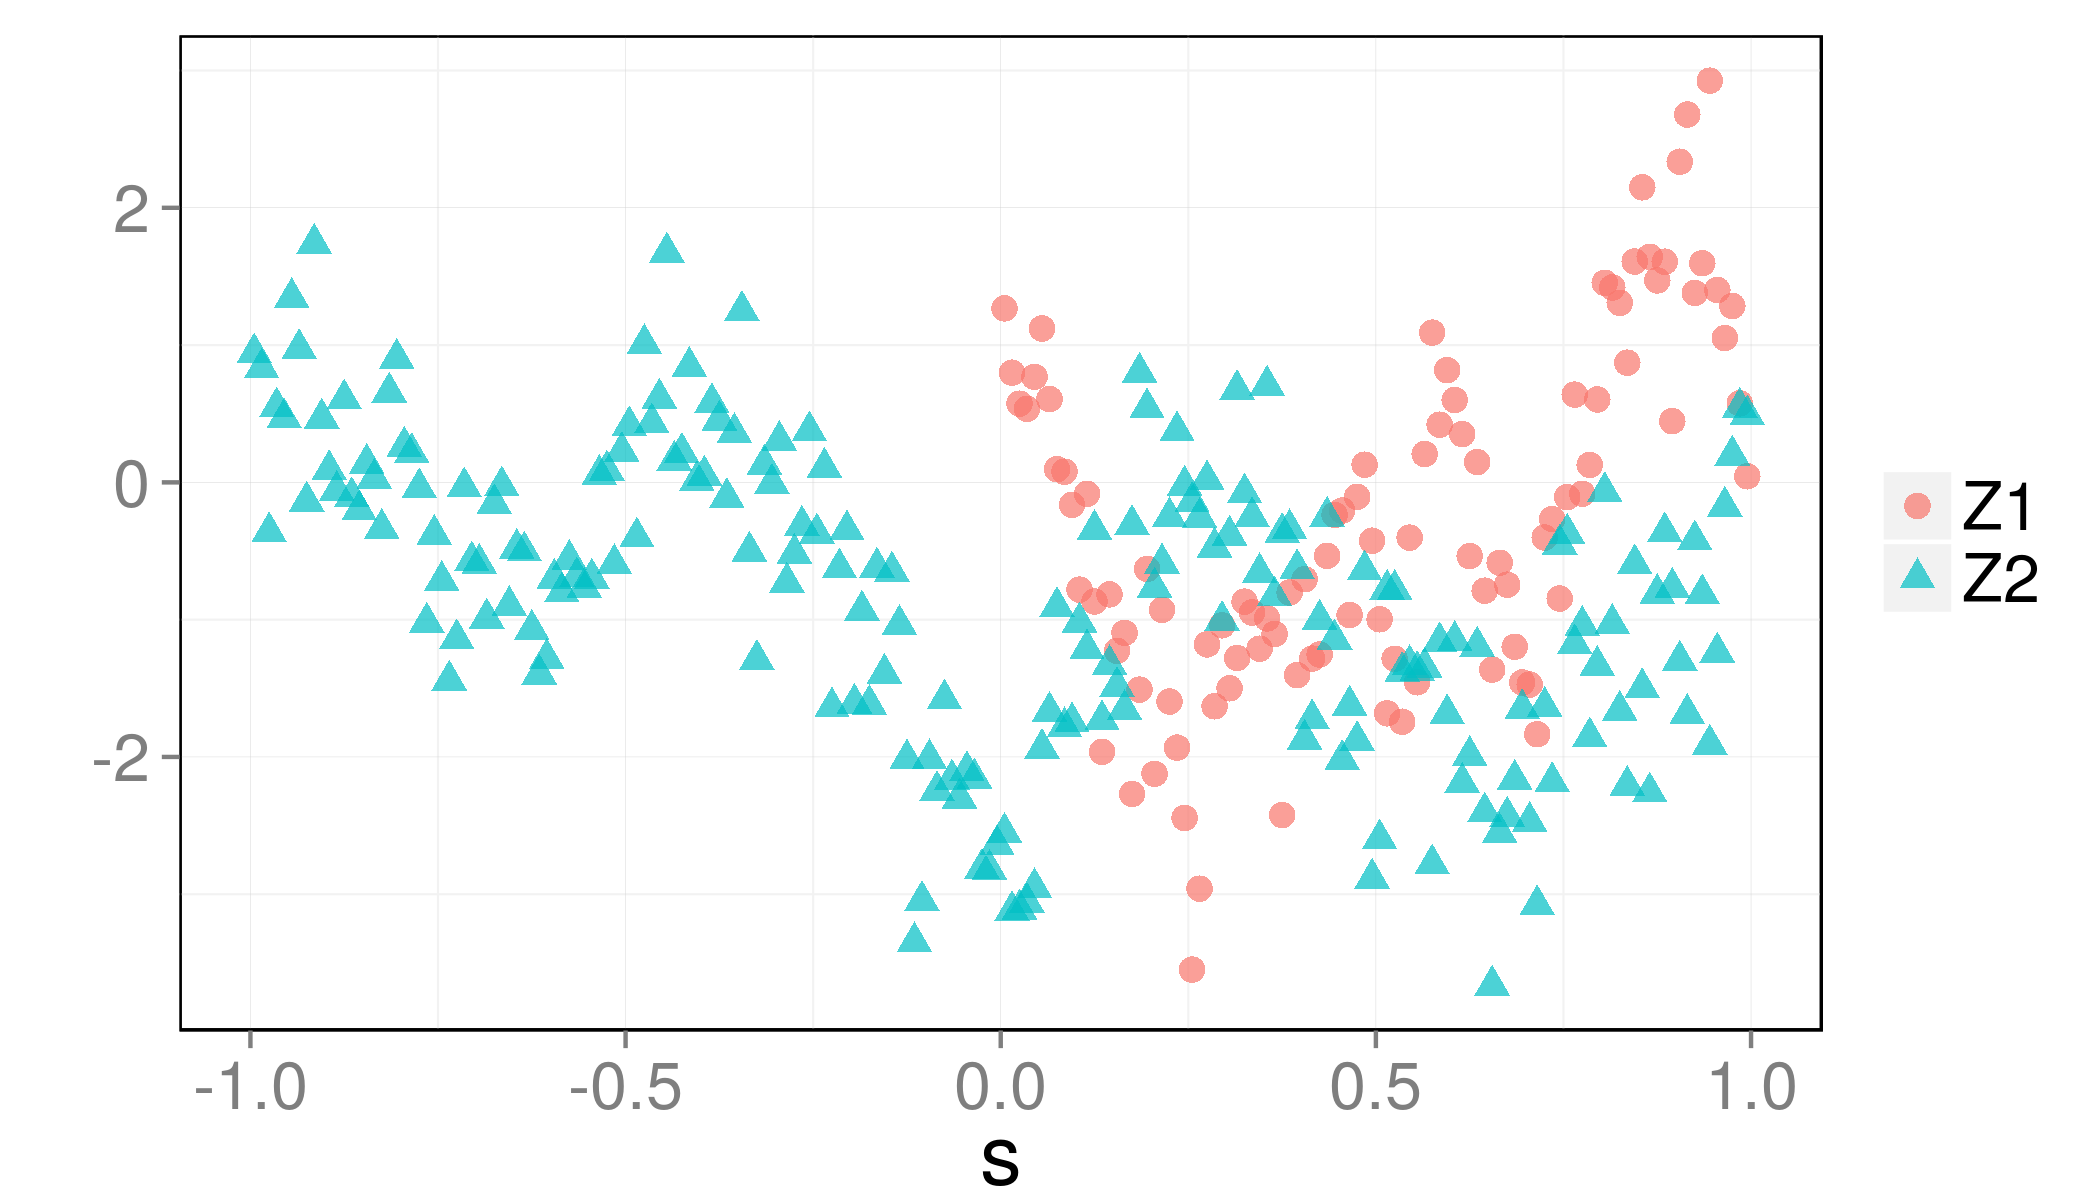
\includegraphics[width=4in]{./sim_obs.png}
\end{center}
\end{frame}

% ###################

\begin{frame}
\frametitle{Cokriging and kriging predictors}
Observations on the first spatial variable are non-existent in the left-hand half of $D$, but \textcolor{red}{cokriging based on all observations} captures the spatial variability over all of $D$.
\vspace{-.5cm}
\begin{center}
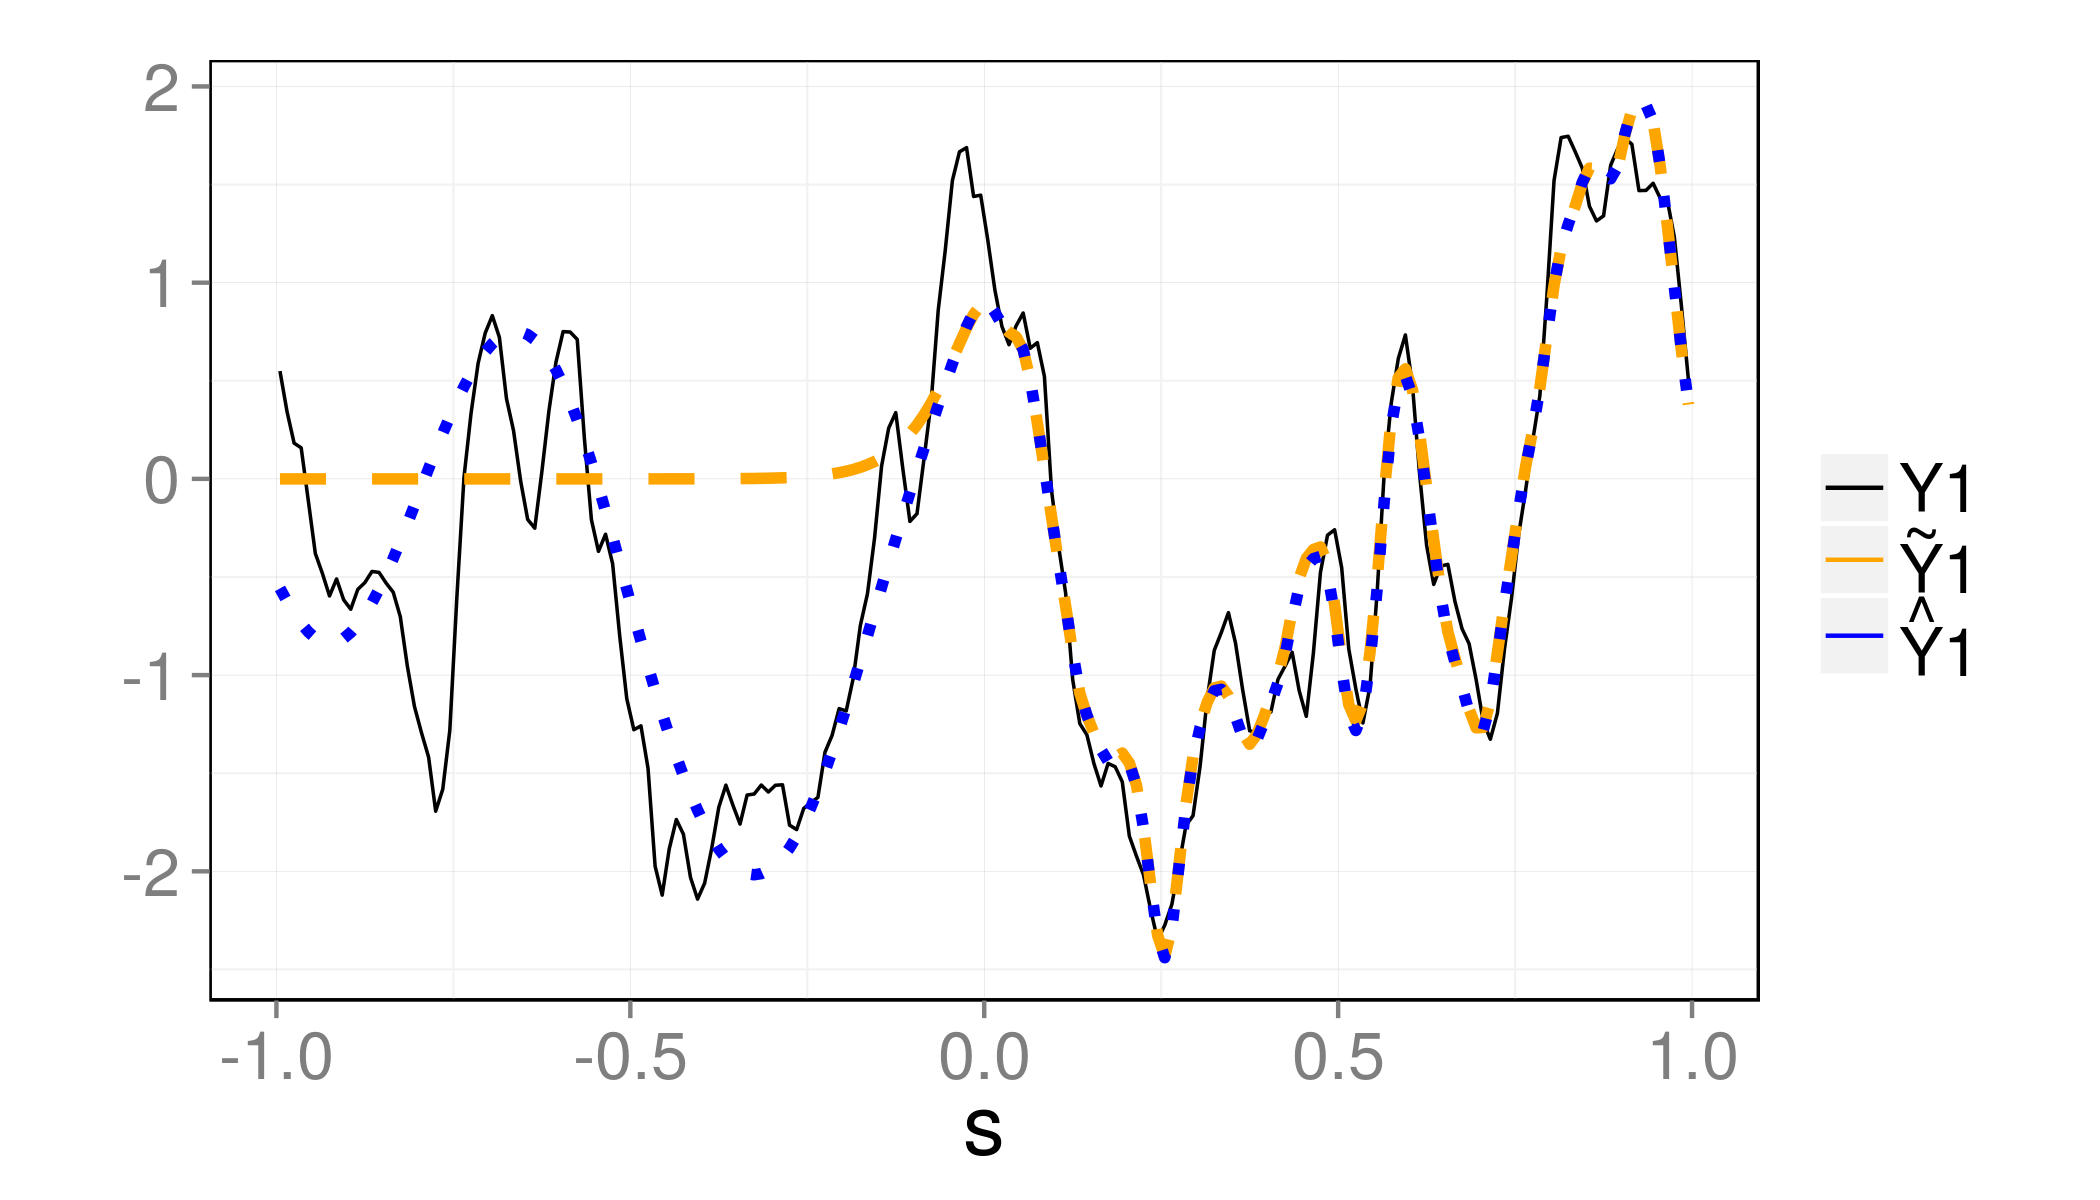
\includegraphics[width=4in]{./sim_est.png}
\end{center}
\end{frame}

% ###################

\begin{frame}
\frametitle{Is the bivariate model always valid?}

\begin{itemize}
\item $C_{11}(\cdot,\cdot)$ and $C_{2|1}(\cdot,\cdot)$ are nnd. Then $C_{22}(\cdot,\cdot)$ is nnd (recall its expression as a quadratic form).
\item $C_{12}(\svec,\uvec) = C_{21}(\uvec,\svec)$; this is \textcolor{red}{not} symmetry, and it trivially holds \\for all $\s,\u$.
\item We now show that \textcolor{red}{CCFM is nnd}. That is, for any $n_1,n_2$ such that $n_1 + n_2 > 0$, any locations $\{\svec_{1k}\}, \{\svec_{2l}\}$, and any real numbers $\{a_{1k}\},\{a_{2l}\}$, we show that

\small
\begin{align*}
 & \var\left(\sum_{k=1}^{n_1}{a_{1k}Y_1(\s_{1k})}+\sum_{l=1}^{n_2}{a_{2l}Y_2(\s_{2l})}\right) \\ &=\sum_{k=1}^{n_1}\sum_{k'=1}^{n_1} a_{1k}a_{1k'}C_{11}(\s_{1k},\s_{1k'})+\sum_{l=1}^{n_2}\sum_{l'=1}^{n_2} a_{2l}a_{2l'}C_{22}(\s_{2l},\s_{2l'}) \\
  &+\sum_{k=1}^{n_1}\sum_{l'=1}^{n_2} a_{1k}a_{2l'}C_{12}(\s_{1k},\s_{2l'})+\sum_{l=1}^{n_2}\sum_{k'=1}^{n_1} a_{2l}a_{1k'}C_{21}(\s_{2l},\s_{1k'})~ \textcolor{red}{\ge 0}.
\end{align*}

\normalsize
\end{itemize}
\end{frame}

% ###################

\begin{frame}
\frametitle{CCFM is nonnegative-definite: Proof}

\begin{itemize}
\item It is straightforward to show that
\begin{align*}
& \var\left(\sum_{k=1}^{n_1}{a_{1k}Y_1(\s_{1k})}+\sum_{l=1}^{n_2}{a_{2l}Y_2(\s_{2l})}\right)\\
&= \sum_{l=1}^{n_2}\sum_{l'=1}^{n_2}a_{2l}a_{2l'}\textcolor{red}{C_{2\mid 1}(\s_{2l},\s_{2l'})}+\int_D \int_D{\red{a(\s)a(\u)}}C_{11}(\s,\u)\,\d\s\d\u,
\end{align*}
where for $\delta(\cdot)$ the Dirac delta function,
\begin{equation*}
a(\s)\equiv \sum_{k=1}^{n_1}a_{1k}\delta(\s-\s_{1k})+\sum_{l=1}^{n_2}a_{2l}b(\s_{2l},\s);\quad \s\in \RR^d.
\end{equation*}
Since $C_{11}(\cdot,\cdot)$ and $C_{2|1}(\cdot,\cdot)$ are nnd by assumption, the right-hand side is $\textcolor{red}{\geq0}$.
\end{itemize}
\end{frame}

% ###################

\begin{frame}
\frametitle{Beyond bivariate}

\begin{itemize}
\item For $p\geq2$, $[Y_1(\cdot),\dots,Y_p(\cdot)]$ can be decomposed as,
$$
[Y_1(\cdot)][Y_2(\cdot)|Y_1(\cdot)]\ldots[Y_p(\cdot) \mid  Y_{p-1}(\cdot),Y_{p-2}(\cdot),\dots,Y_1(\cdot)].
$$ \pause
\vspace{-.6cm}
\item Assume the conditional expectation for the $q$-th term is, for $\s\in D$,
\begin{equation*}
\E(Y_q(\svec) \mid  \{Y_r(\cdot) : r = 1,\dots,q-1\}) \equiv \sum_{r = 1}^{q-1} \int_D \textcolor{red}{b_{qr}(\svec,\v)}Y_r(\v) \intd \v,
\end{equation*}
where $\{b_{qr}(\cdot,\cdot):r=1,\ldots,q-1;q=2,\ldots,p\}$ are integrable. \pause
\item Assume the conditional covariance for the $q$-th term is, for $\s,\u\in\mathbb{R}^d$,
\begin{align*}
\cov(Y_q(\svec), Y_q(\uvec) \mid  \{Y_r(\cdot) : r = 1,\dots,(q-1)\}) \equiv \textcolor{red}{C_{q \mid  (r < q)}(\svec,\uvec)}.
\end{align*}
\end{itemize}
\end{frame}

% ###################

\begin{frame}
\frametitle{Is the multivariate model always valid?}

We show that the $p$-variate process is well defined, by induction:
\begin{itemize}
  \item For nnd $C_{11}$ and $C_{2|1}$, the bivariate process is valid.
  \item Assume that the $(p-1)$-variate process is valid.
  \item Show that the $p$-variate process is valid. For any $n$'s, $\s$'s, and $a$'s,
\end{itemize}

\vspace{-0.3in}
\begin{align*}
\var\left(\sum_{q=1}^p \sum_{m=1}^{n_q} a_{qm}Y_q(\svec_{qm})\right)=& \sum_{m=1}^{n_p}\sum_{m'=1}^{n_p}a_{pm}a_{pm'}\textcolor{red}{C_{p \mid  (q < p)}(\svec_{pm},\svec_{pm'})} \\
&+ \sum_{q=1}^{p-1}\sum_{r=1}^{p-1}\int_D\int_D\red{a_q(\svec)a_r(\uvec)}C_{qr}(\svec,\uvec)\intd \svec \intd \uvec,
\end{align*}
where for $\delta(\cdot)$ the Dirac delta function and for $\s\in\mathbb{R}^d$,
\begin{equation*}
a_q(\svec) \equiv \left(\sum_{k=1}^{n_q}a_{qk}\delta(\svec - \svec_{qk}) + \sum_{m=1}^{n_p}a_{pm}b_{pq}(\svec_{pm},\svec)\right).
\end{equation*}
\end{frame}

% ###################

\begin{frame}
\frametitle{Generalisations}
\vspace{-1cm}
The following families of multivariate spatial processes contain classes that are special cases of models defined by the conditional approach:

\begin{itemize}
\item The parsimonious Mat{\'e}rn model of \cite{Gneitingetal2010}.\vfil
%\item The full Mat{\'e}rn model of \cite{Gneitingetal2010}.\vfil
\item The linear model of coregionalisation, used for example by \cite{Wackernagel1995}.\vfil
\item The moving average model of \cite{verHoef_1998}.\vfil
\item The shifted models of Ver Hoef and Cressie, Christensen and Amemiya, and Li and Zhang (see earlier slide: Bivariate spatial \\models with asymmetry).
\end{itemize}
\vfill
\end{frame}

% ###################

\begin{frame}
\frametitle{Graph structure}

\begin{itemize}
\item Directed acyclic graphs on the variables define a partial order that specifies which conditional covariances, $\{C_{q|(r<q)}\}$, appear in the model.
\item Computationally efficient algorithms are available for directed acyclic graphs.
\end{itemize}
 Examples include:

\begin{figure}[!t]
\begin{center}

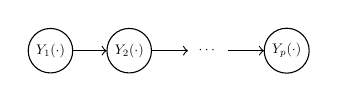
\begin{tikzpicture}[scale=0.5,every node/.style={transform shape}]
%[inner sep=1mm]
[line width=1pt]

\path (0,0) node (Y1) [shape=circle, minimum size=1cm,draw] {$Y_1(\cdot)$};
\path (2,0) node (Y2) [shape=circle, minimum size=1cm,draw] {$Y_2(\cdot)$};
\path (4,0) node (dots) [shape=circle, minimum size=1cm] {$\cdots$};
\path (6,0) node (Yp)  [shape=circle, minimum size=1cm,draw] {$Y_p(\cdot)$};

\draw [->] (Y1) to (Y2);
\draw [->] (Y2) to (dots);
\draw [->] (dots) to (Yp);

\end{tikzpicture}
%\caption{Ordered nodes}\label{fig:exchangeable1}
\end{center}
\end{figure}

\begin{figure}[!t]
\begin{center}

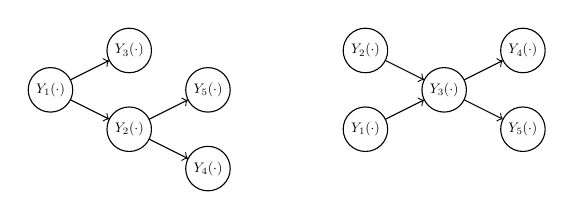
\begin{tikzpicture}[scale=0.5,every node/.style={transform shape}]
%[inner sep=1mm]
[line width=1pt]

\path (0,0) node (Y1) [shape=circle, minimum size=1cm,draw] {$Y_1(\cdot)$};
\path (2,-1) node (Y3) [shape=circle, minimum size=1cm,draw] {$Y_2(\cdot)$};
\path (2,1) node (Y2) [shape=circle, minimum size=1cm,draw] {$Y_3(\cdot)$};
\path (4,-2) node (Y4)  [shape=circle, minimum size=1cm,draw] {$Y_4(\cdot)$};
\path (4,0) node (Y5)  [shape=circle, minimum size=1cm,draw] {$Y_5(\cdot)$};

\draw [->] (Y1) to (Y2);
\draw [->] (Y1) to (Y3);
\draw [->] (Y3) to (Y4);
\draw [->] (Y3) to (Y5);


\path (8,-1) node (Y1b) [shape=circle, minimum size=1cm,draw] {$Y_1(\cdot)$};
\path (8,1) node (Y2b) [shape=circle, minimum size=1cm,draw] {$Y_2(\cdot)$};
\path (10,0) node (Y3b) [shape=circle, minimum size=1cm,draw] {$Y_3(\cdot)$};
\path (12,1) node (Y4b)  [shape=circle, minimum size=1cm,draw] {$Y_4(\cdot)$};
\path (12,-1) node (Y5b)  [shape=circle, minimum size=1cm,draw] {$Y_5(\cdot)$};

\draw [->] (Y1b) to (Y3b);
\draw [->] (Y2b) to (Y3b);
\draw [->] (Y3b) to (Y4b);
\draw [->] (Y3b) to (Y5b);


\end{tikzpicture}
%\caption{Trees and polytrees}
\end{center}

\end{figure}

\end{frame}

% ###################

\begin{frame}
\frametitle{Model flexibility}

\begin{figure}[!t]
\begin{center}

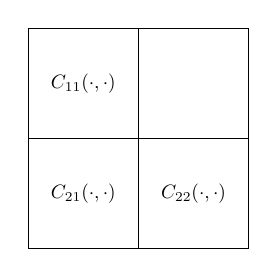
\begin{tikzpicture}[scale=0.7,every node/.style={transform shape}]
%[inner sep=1mm]
[line width=1pt]

\path (0,0) node (X11) [shape=rectangle, minimum size=2cm,draw] {$C_{11}(\cdot,\cdot)$};
\path (2,0) node (X12) [shape=rectangle, minimum size=2cm,draw] {};
\path (0,-2) node (X21) [shape=rectangle, minimum size=2cm,draw] {$C_{21}(\cdot,\cdot)$};
\path (2,-2) node (X22)  [shape=rectangle, minimum size=2cm,draw] {$C_{22}(\cdot,\cdot)$};


\end{tikzpicture}
\end{center}
\end{figure}
\textcolor{red}{Bivariate system}: We need to specify \textcolor{red}{three} marginal/cross-covariance functions. Recall that $C_{12}(\s,\u)=C_{21}(\u,\s)$, which is not asymmetry.

Available building blocks using the conditional approach: \textcolor{red}{Three} functions, $C_{11}(\cdot,\cdot)$, $C_{2\mid 1}(\cdot,\cdot)$, $b(\cdot,\cdot)$.

\end{frame}

% ###################

\begin{frame}
\frametitle{Model flexibility, ctd}
\vspace{-0.5cm}
\begin{figure}[!t]
\begin{center}

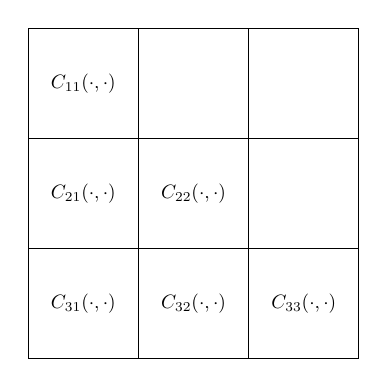
\begin{tikzpicture}[scale=0.7,every node/.style={transform shape}]
%[inner sep=1mm]
[line width=1pt]

\path (0,0) node (X11) [shape=rectangle, minimum size=2cm,draw] {$C_{11}(\cdot,\cdot)$};
\path (2,0) node (X12) [shape=rectangle, minimum size=2cm,draw] {};
\path (4,0) node (X13) [shape=rectangle, minimum size=2cm,draw] {};
\path (0,-2) node (X21) [shape=rectangle, minimum size=2cm,draw] {$C_{21}(\cdot,\cdot)$};
\path (2,-2) node (X22)  [shape=rectangle, minimum size=2cm,draw] {$C_{22}(\cdot,\cdot)$};
\path (4,-2) node (X23)  [shape=rectangle, minimum size=2cm,draw] {};
\path (0,-4) node (X31) [shape=rectangle, minimum size=2cm,draw] {$C_{31}(\cdot,\cdot)$};
\path (2,-4) node (X32)  [shape=rectangle, minimum size=2cm,draw] {$C_{32}(\cdot,\cdot)$};
\path (4,-4) node (X33)  [shape=rectangle, minimum size=2cm,draw] {$C_{33}(\cdot,\cdot)$};


\end{tikzpicture}
\end{center}
\end{figure}
\textcolor{red}{Trivariate system}: Need to specify \textcolor{red}{six} marginal/cross-covariance functions. Recall that $C_{ij}(\s,\u)=C_{ji}(\u,\s)$.

Available building blocks using the conditional approach: \textcolor{red}{Six} functions, $C_{11}(\cdot,\cdot)$, $C_{2\mid 1}(\cdot,\cdot)$, $C_{3|1,2}(\cdot,\cdot)$, $b_{21}(\cdot,\cdot)$, $b_{31}(\cdot,\cdot)$, $b_{32}(\cdot,\cdot)$.

\end{frame}

% ###################

%\subsection{Min-max temperature dataset}

\begin{frame}
\frametitle{Min-max temperatures in Colorado, USA}

\begin{itemize}
\item Datatset: Minimum and maximum temperatures taken on September 19, 2004 in the state of Colorado, USA.
\item Data come from 94 measurement stations (collocated measurements); our data are residuals $\mathbf{Z}_1$(min. temp.) and $\mathbf{Z}_2$(max. temp.) obtained by subtraction of the respective statewide means.
\item The maximum\hyp{}temperature residual process, occurring later in the afternoon ($Y_2(\cdot)$), is highly dependent on the minimum\hyp{}temperature residual process, occurring in the early-morning hours ($Y_1(\cdot)$).
\item We fit three models and compare them using DIC:
\begin{equation*}
\begin{array}{ll}
\textrm{\textcolor{red}{Model 1}:} &b_o(\h) \equiv 0 \mbox{ (i.e., independence)}\\
\textrm{\textcolor{red}{Model 2}:} &b_o(\h) \equiv A\delta(\h) \mbox{ (i.e., pointwise dependence)}\\
\textrm{\textcolor{red}{Model 3}:} &b_o(\h) \equiv \left\{\begin{array}{ll} A\{1 - (\|\h - \Deltab\|/r)^2\}^2, & \| \h - \Deltab\| \le r \\ 0, & \textrm{otherwise}. \end{array} \right.
\end{array}
\end{equation*}
\end{itemize}
\end{frame}

% ###################

\begin{frame}
\frametitle{Discretisations}
\begin{itemize}
\item Consider a discretisation of $Y_1(\cdot)$ and $Y_2(\cdot)$; call the resulting $n$-dimensional ($n=968$) vectors $\Yvec_1$ and $\Yvec_2$ respectively, and define $\Yvec \equiv (\Yvec_1^{\prime},\Yvec_2^{\prime})'$. The 188-dimensional data vector is $\Zvec \equiv (\Zvec_1^{\prime},\Zvec_2^{\prime})'$ at 94 locations:
\end{itemize}

\vspace{-0.2in}
\begin{center}
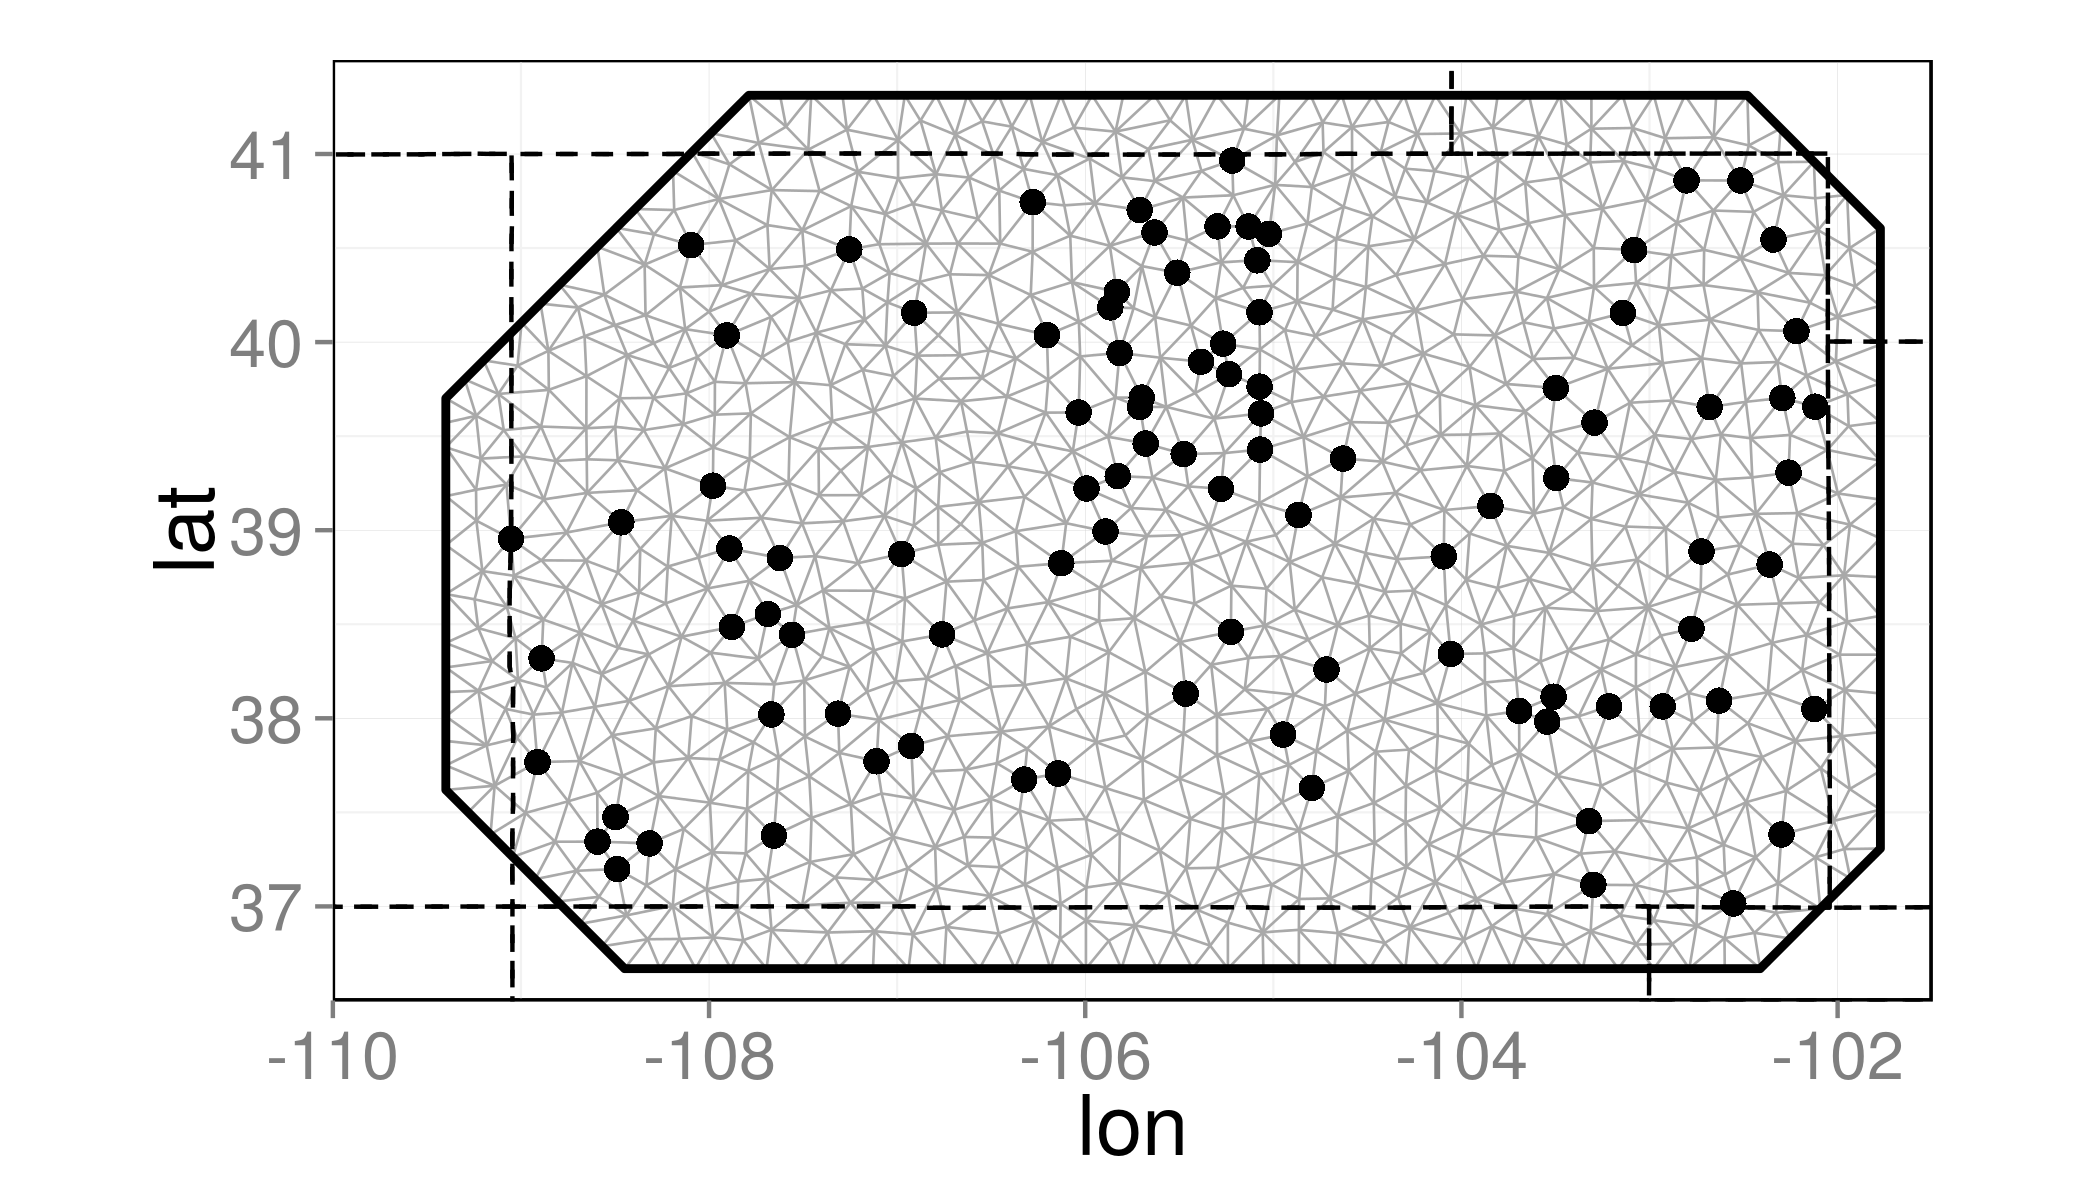
\includegraphics[width=4in]{meshplot.png}
\end{center}

\end{frame}

% ###################


\begin{frame}
\frametitle{Numerical integrations}

\vspace{-.8cm}
\begin{center}
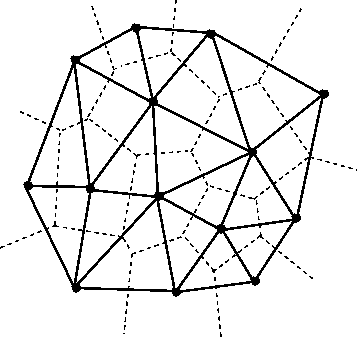
\includegraphics[width=2in]{vor3.png}
\end{center}
\vspace{-.5cm}
\begin{align*}
\mbox{Approximate }&\displaystyle \E\left(Y_2(\s)\mid Y_1(\cdot)\right)=\int_D{b(\s,\v)Y_1(\v)\,\d \v};\,\,\s\in D,\,\mbox{ by}\\
&\E(Y_2(\svec_l) \mid  Y_1(\cdot)) \simeq \sum_{k=1}^{n} A_k b(\svec_l,\v_k)Y_1(\v_k),
\end{align*}
where $\{A_k:k=1,\ldots,968\}$ are the polygonal-tessellation areas.
\end{frame}

% ###################

\begin{frame}
\frametitle{Full model}

\begin{itemize}
\item Data model:
\begin{align*}
\left.\begin{pmatrix} \Zvec_1 \\ \Zvec_2 \end{pmatrix}
\right|
\begin{pmatrix} \Yvec_1 \\ \Yvec_2 \end{pmatrix} \hspace{-0.02in} ,\thetab
\sim
\mathcal{N}\left(
\begin{pmatrix} \Dmat\Yvec_1 \\ \Dmat\Yvec_2 \end{pmatrix}  \hspace{-0.02in}, \sigma^2_\varepsilon\begin{pmatrix} \Imat & \rho_\varepsilon\Imat \\ \rho_\varepsilon\Imat & \Imat \end{pmatrix}
\right),
\end{align*}
where $\Dmat$ is a $94\times 968$ incidence matrix and $\thetab$ includes $\sigma^2_\varepsilon$ and $\rho_\varepsilon$.
\item Process model:
\begin{equation*}
\left.\begin{pmatrix} \Yvec_1 \\ \Yvec_2 \end{pmatrix}\right| \thetab \sim \mathcal{N}
\left(
\begin{pmatrix} \bzero \\ \bzero \end{pmatrix},
\begin{pmatrix}
\bSigma_{11} & \bSigma_{11}\Bmat' \\
\Bmat \bSigma_{11} & \Bmat \bSigma_{11}\Bmat' + \bSigma_{2|1}
\end{pmatrix}
\right),
\end{equation*}
\noindent where $\mathbf{B}$ (\textcolor{red}{interaction matrix}), $\bSigma_{11}$ (\textcolor{red}{marginal covariance matrix}), and $\bSigma_{2|1}$ (\textcolor{red}{conditional covariance matrix}) are $968\times 968$ matrices that depend on parameters included in $\thetab$.
\item Parameter model: see \texttt{https://github.com/andrewzm/bicon}
\end{itemize}
\end{frame}

% ###################

\begin{frame}
\frametitle{We have many unknown parameters!}
\vspace{-.5cm}
Assume $C_{11}(\cdot)$ and $C_{2|1}(\cdot)$ are equally smooth Mat{\'e}rn covariance functions with parameters ($\nu_{11}=1.5, \kappa_{11}, \sigma_{11}^2$) and ($\nu_{2|1}=1.5,\kappa_{2|1},\sigma_{2|1}^2$), respectively. Here we show our (Bayesian) inference on the \textcolor{red}{scale parameters} only.
\small
\begin{center}
\begin{tabular} {cccc}
  { Parameter} 	& {Model 1} 	& {Model 2} & {Model 3} 			 \\
  $\sigma_\varepsilon^2$&  x & x & x \\
  $\rho_\varepsilon$&  x & x & x \\
  $\sigma^2_{11}$& x & x & x \\
  $\sigma^2_{2|1}$& x & x & x \\
  $\textcolor{red}{\kappa_{11}}$&0.98 (0.76, 1.22)&1 (0.8, 1.26)&\textcolor{red}{1.03 (0.83, 1.25)}\\
  $\textcolor{red}{\kappa_{2|1}}$&0.76 (0.56, 1)&0.62 (0.46, 0.81)&\textcolor{red}{3.65 (1.16, 6.72)}\\
  $A$&& x & x \\
  $r$&&& x \\
  $\Delta_1$&&& x\\
  $\Delta_2$&&& x \\
  &&&\\
  $DIC$&992.45&985.17&\textcolor{red}{982.45}
\end{tabular}
\end{center}
\normalsize
\end{frame}

% ###################

\begin{frame}
\frametitle{Posterior mean field: Minimum temperature}

\begin{figure}
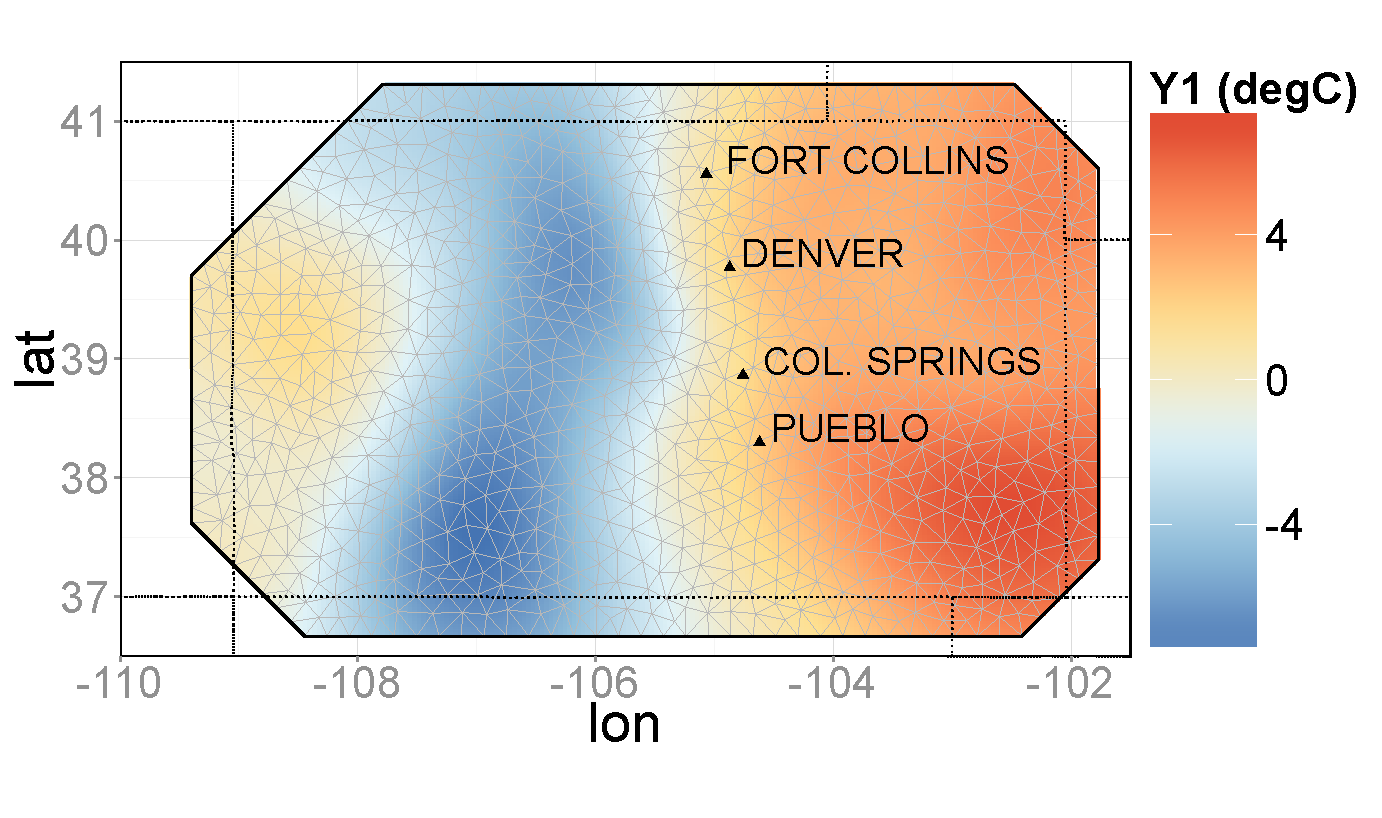
\includegraphics[width=3in]{Fig3a1.png}
\end{figure}
\vspace{-.5cm}
Interpolated map of predicted (residual) \textcolor{red}{minimum temperature}, $\E(\Yvec_1 \mid  \Zvec_1,\Zvec_2)$, in degrees Celsius (degC).
\end{frame}

% ###################

\begin{frame}
\frametitle{Posterior mean field: Maximum temperature}
\begin{figure}
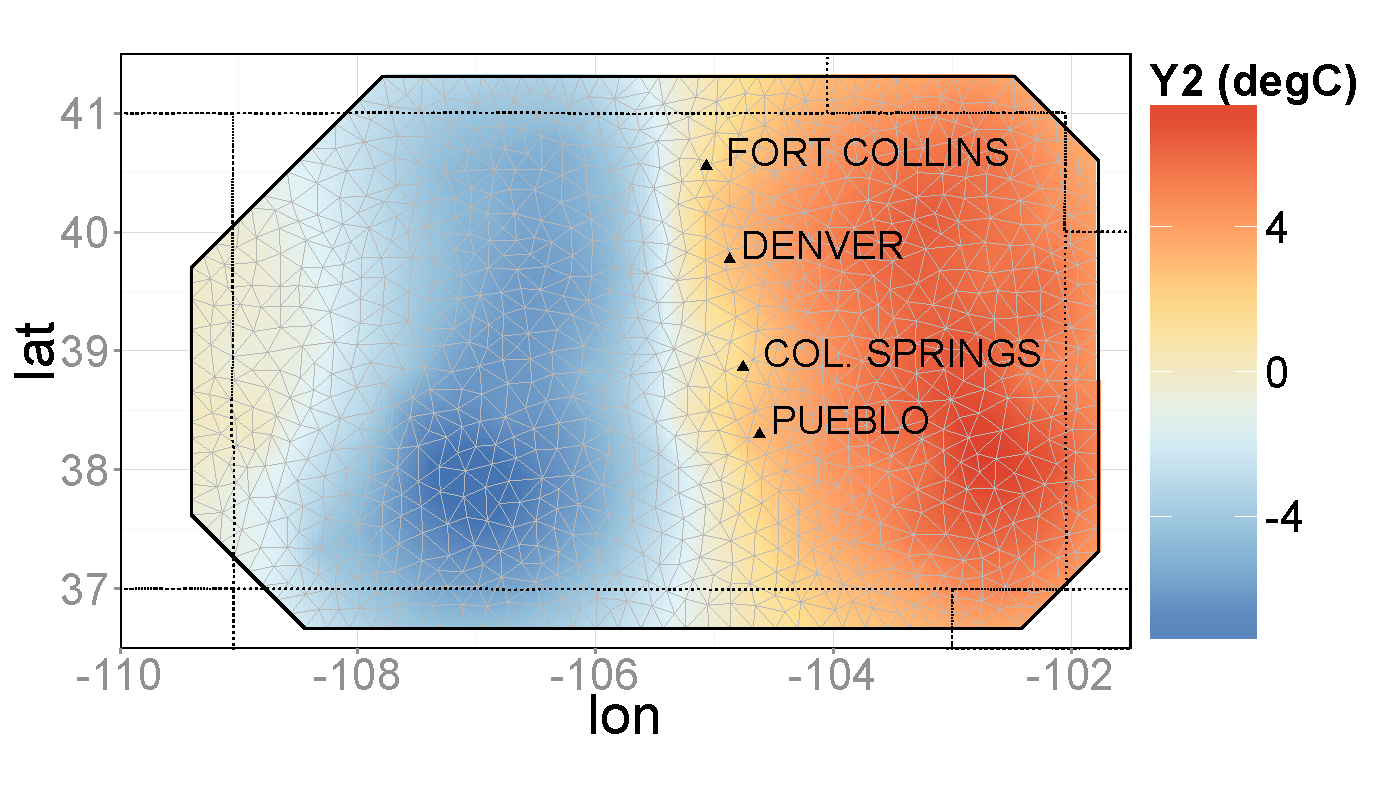
\includegraphics[width=3in]{Fig3a2.png}
\end{figure}
\vspace{-.5cm}
Interpolated map of predicted (residual) \textcolor{red}{maximum temperature}, $\E(\Yvec_2 \mid  \Zvec_1,\Zvec_2)$, in degrees Celsius (degC).
\end{frame}

% ###################

\begin{frame}
\frametitle{Interaction function for Model 3}
\vspace{-0.2in}
\begin{figure}
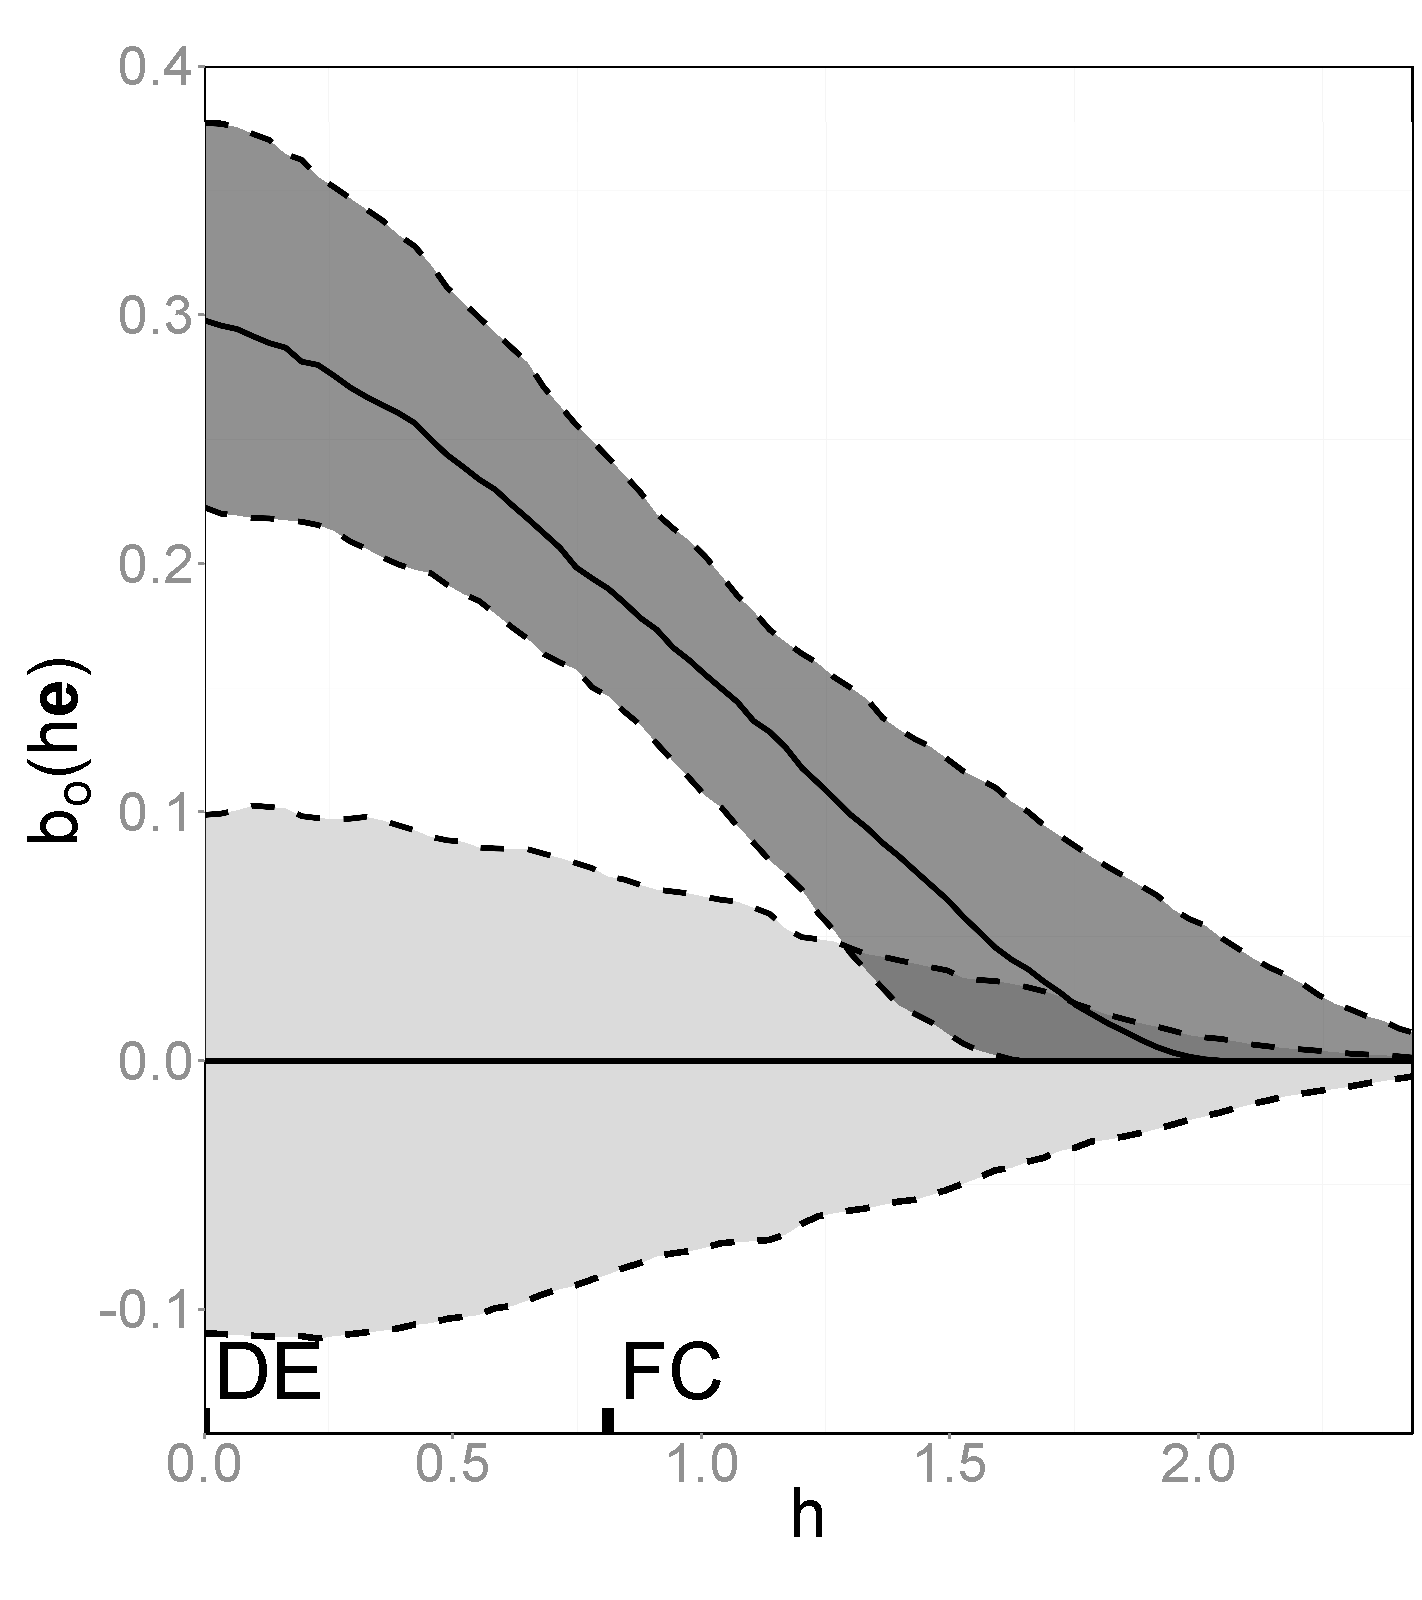
\includegraphics[width=2in]{Fig3b.png}
\end{figure}
\vspace{-.5cm}
\small{Prior (light grey) and posterior (dark grey) median (solid line) and interquartile ranges (enclosed by dashed lines) of \textcolor{red}{$b_o(\cdot)$ from Model 3}, along a unit vector $\mathbf{e}$ originating at Denver (DE) in the direction of Fort Collins (FC).}
\end{frame}

% ###################


\begin{frame}
\frametitle{Conclusions}

\begin{itemize}
\item \textcolor{red}{Bivariate and multivariate spatial models} often appear in environmental studies. For convenience, one or more of these variables are often ``explained away'' prior to commencing a univariate spatial analysis. We wish to avoid this by providing a methodology for building flexible (e.g., no symmetry constraint) multivariate spatial models whose CCFMs are nnd.
\item The \textcolor{red}{conditional approach} allows for a (very) flexible model class through the use of integrable \textcolor{red}{interaction functions} that can be arbitrarily complex.
\item For large, non-Gaussian systems, computational efficiency is key.
\item Slides and reproducible code available at \texttt{https://github.com/andrewzm/bicon}.
\end{itemize}
\end{frame}

\small

\begin{frame}%[allowframebreaks]
\frametitle{References}

\bibliographystyle{apa}
\vspace{-1cm}
\scriptsize{
\bibliography{Bibliography}}


\end{frame}

\end{document}

